% Template for a Computer Science Tripos Part II project dissertation
\documentclass[12pt,a4paper,oneside,openright]{report}

\usepackage{adjustbox}
\usepackage[indent=0pt,skip=10pt]{parskip}
\usepackage[pdfborder={0 0 0}]{hyperref}    % turns references into hyperlinks
\usepackage[margin=25mm]{geometry}  % adjusts page layout
\usepackage{graphicx}  % allows inclusion of PDF, PNG and JPG images
\usepackage{verbatim}
\usepackage{docmute}   % only needed to allow inclusion of proposal.tex
\usepackage[utf8]{inputenc}
\usepackage{mathtools}
\usepackage{changepage}
\usepackage{url}
\usepackage{blindtext}
\usepackage[dvipsnames]{xcolor}
\usepackage{qtree}
\usepackage{tipa}
\usepackage{dirtree}
\usepackage{svg}
\usepackage[format=hang,labelfont=bf]{caption}
\usepackage{subcaption}
\usepackage[algoruled,vlined]{algorithm2e}
\usepackage{fancyref}
\usepackage{pifont}
\usepackage{soul}

\usepackage[sorting=none]{biblatex}
\bibliography{refs}

%\raggedbottom                           % try to avoid widows and orphans
\sloppy
\clubpenalty1000%
\widowpenalty1000%

\renewcommand{\baselinestretch}{1.1}    % adjust line spacing to make
                                        % more readable
\newcommand{\vital}{\colorbox{Bittersweet}{\textcolor{White}{Vital}}}
\newcommand{\veryhard}{\colorbox{BrickRed}{\textcolor{White}{Very Challenging}}}

\newcommand{\hard}{\colorbox{RedOrange}{Challenging}}
\newcommand{\high}{\colorbox{RedOrange}{High}}

\newcommand{\medium}{\colorbox{Dandelion}{Intermediate}}
\newcommand{\interm}{\colorbox{Dandelion}{Intermediate}}

\newcommand{\low}{\colorbox{LimeGreen}{Low}}
\newcommand{\easy}{\colorbox{LimeGreen}{Simpler}}

\newcommand{\extension}{\colorbox{Violet}{\textcolor{White}{\textsc{Extension}}}}

\newcommand{\user}{User Study}
\newcommand{\inspect}{Inspection}

\newcommand{\element}{\texttt{Element}}
\newcommand{\pos}{\texttt{Pos}}
\newcommand{\boxT}{\texttt{Box}}
\newcommand{\window}{\texttt{Window}}
\newcommand{\canvas}{\texttt{Canvas}}
\newcommand{\controlbar}{\texttt{ControlBar}}
\newcommand{\timebar}{\texttt{TimeBar}}
\newcommand{\button}{\texttt{Button}}
\newcommand{\playable}{\texttt{Playable}}
\newcommand{\sample}{\texttt{Sample}}
\newcommand{\effect}{\texttt{Effect}}
\newcommand{\capsule}{\texttt{Capsule}}
\newcommand{\mouse}{\texttt{Mouse}}
\newcommand{\labelT}{\texttt{Label}}

\newcommand{\usability}{\textbf{usability}}
\newcommand{\clarity}{\textbf{clarity}}
\newcommand{\expressiveness}{\textbf{expressiveness}}
\newcommand{\Usability}{\textbf{Usability}}
\newcommand{\Clarity}{\textbf{Clarity}}
\newcommand{\Expressiveness}{\textbf{Expressiveness}}

\newcommand{\quoteT}[1]{``\textit{#1}"}

\newcommand{\statement}[1]{\vspace{1em}
\hrule
\begin{center}
#1
\end{center}
\vspace{1em}
\hrule}

\newcommand{\checkmark}{\ding{51}}

\newcommand*{\fancyrefalglabelprefix}{alg}

\newcommand*{\fancyrefappendixlabelprefix}{appendix}

\frefformat{main}{\fancyrefalglabelprefix}{\textbf{algorithm~#1}}
\Frefformat{main}{\fancyrefalglabelprefix}{\textbf{Algorithm~#1}}

\frefformat{main}{\fancyrefappendixlabelprefix}{\textbf{appendix~#1}}
\Frefformat{main}{\fancyrefappendixlabelprefix}{\textbf{Appendix~#1}}

\frefformat{main}{\fancyreffiglabelprefix}{\textbf{figure~#1}}
\Frefformat{main}{\fancyreffiglabelprefix}{\textbf{Figure~#1}}

\frefformat{main}{\fancyrefseclabelprefix}{\S#1}
\Frefformat{main}{\fancyrefseclabelprefix}{\S#1}

\frefformat{main}{\fancyrefchaplabelprefix}{\textbf{chapter~#1}}
\Frefformat{main}{\fancyrefchaplabelprefix}{\textbf{Chapter~#1}}

% https://www.overleaf.com/learn/how-to/Is_there_a_way_to_run_a_word_count_that_doesn%27t_include_LaTeX_commands%3F
\newcommand{\detailtexcount}[1]{%
  \immediate\write18{texcount -merge -sum -q #1.tex output.bbl > #1.wcdetail }%
  \verbatiminput{#1.wcdetail}%
}

% https://tex.stackexchange.com/a/63393/266746
\makeatletter
\def\@makechapterhead#1{%
  \vspace*{10\p@}% 50->10
  {\parindent \z@ \raggedright \normalfont
    \ifnum \c@secnumdepth >\m@ne
        \huge\bfseries \@chapapp\space \thechapter
        \par\nobreak
        \vskip 20\p@
    \fi
    \interlinepenalty\@M
    \Huge \bfseries #1\par\nobreak
    \vskip 20\p@% 40->20
  }}
\def\@makeschapterhead#1{%
  \vspace*{10\p@}% %%% 50->10
  {\parindent \z@ \raggedright
    \normalfont
    \interlinepenalty\@M
    \Huge \bfseries  #1\par\nobreak
    \vskip 20\p@% 40->20
  }}
\makeatother

\begin{document}
%TC:ignore
% Change these

\newcommand{\mcandidate}{2416B}
\newcommand{\mfullname}{Jude Howard-Gluckstein Tyrrell}
\newcommand{\mcollege}{Homerton College}
\newcommand{\mtitle}{Notation for Phonological Audio Composition}
\newcommand{\mexamination}{Computer Science Tripos -- Part II}
\newcommand{\mdate}{May 2023}
\newcommand{\moriginator}{Prof. Alan Blackwell}
\newcommand{\msupervisor}{Prof. Alan Blackwell}
\newcommand{\mwordcount}{10814}
\newcommand{\mlinecount}{0}
% Consent to the dissertation made available to University members
\newcommand{\mconsent}{I am content for my dissertation to be made available to the students and staff of the University.}
% For the Declaration of originality
\newcommand{\msignature}{Jude Tyrrell}


%\detailtexcount{main}

%%%%%%%%%%%%%%%%%%%%%%%%%%%%%%%%%%%%%%%%%%%%%%%%%%%%%%%%%%%%%%%%%%%%%%%%
% Title


\thispagestyle{empty}

\rightline{\LARGE \textbf{\mfullname}}

\vspace*{60mm}
\begin{center}
\Huge
\textbf{\mtitle} \\[5mm]
\mexamination \\[5mm]
\mcollege \\[5mm]
\mdate  % today's date
\end{center}

%%%%%%%%%%%%%%%%%%%%%%%%%%%%%%%%%%%%%%%%%%%%%%%%%%%%%%%%%%%%%%%%%%%%%%%%%%%%%%
% Proforma, table of contents and list of figures

\pagestyle{plain}

\newpage
\newpage
\section*{Declaration of originality}

I, Jude Tyrrell of \mcollege, being a candidate for Part II of the Computer Science Tripos, hereby declare that this dissertation and the work described in it are my own work, unaided except as may be specified below, and that the dissertation does not contain material that has already been used to any substantial extent for a comparable purpose. In preparation of this dissertation I did not use text from AI-assisted platforms generating natural language answers to user queries, including but not limited to ChatGPT. \mconsent

\bigskip
\leftline{Signed \msignature}
\bigskip
\leftline{Date \today}

\chapter*{Proforma}

{\large
\begin{tabular}{ll}
Candidate Number:   & \bf \mcandidate                   \\
Project Title:      & \bf \mtitle                       \\
Examination:        & \bf \mexamination, \mdate         \\
Word Count:         & \bf \mwordcount\footnotemark[1]   \\
Code Line Count:    & \bf \mlinecount                   \\
Project Originator: & \bf \moriginator                  \\
Supervisor:         & \bf \msupervisor                  \\ 
\end{tabular}
}
\footnotetext[1]{This word count was computed
by \TeX count, using the \LaTeX commands \texttt{\textbackslash immediate\textbackslash write18\{texcount -merge -sum -q \#1.tex output.bbl > \#1.wcdetail \}\%
  \textbackslash verbatiminput\{\#1.wcdetail\}\%}}
\stepcounter{footnote}


\section*{Original Aims of the Project}
% At most 100 words
The project aimed to explore the capabilities of computer music through the design and implementation of a novel system for musical expression focused on enabling phonological composition, a style of composition which manipulates the structure of language for musical effect. The system was to be easy to use and accessible for artists, and intuitive in its design.

\section*{Work Completed}
% At most 100 words
The project was a success, producing a computational model of composition, text-based tool and interactive graphical software. The final program, tuPAC, was evaluated to be more intuitive and easier to use than Ableton Live, a popular digital composition tool, when completing tasks that the software was designed to facilitate. This evaluation was done through a user study.

\section*{Special Difficulties}
% At most 100 words
None.

\newpage

\tableofcontents

\newpage
\section*{Acknowledgements}
During the development of the project and the writing of this dissertation, I was supported and helped by many people. In particular, I would like to thank:
\begin{itemize}
\item[--] My supervisor Professor Alan Blackwell for suggesting the project and his advice, suggestions and feedback throughout.
\item[--] Coby O'Brien for inspiring the project, their feedback throughout the project on what is desirable in a project like this, and providing examples of phonological composition.
\item[--] My family and friends for their support.
\item[--] My girlfriend Lizzie and my friends for proofreading this dissertation.
\end{itemize}

%%%%%%%%%%%%%%%%%%%%%%%%%%%%%%%%%%%%%%%%%%%%%%%%%%%%%%%%%%%%%%%%%%%%%%%
% now for the chapters

\pagestyle{headings}


%TC:macro \footnote [text]

%TC:endignore
\chapter{Introduction}
Since the earliest development of electronic devices, people have utilised them extensively in the creation of art, especially music. From the theremin to synthesizers to trackers and modern day \textbf{Digital Audio Workstations} (hereafter referred to as DAWs), electronics have enabled people to compose music more easily than ever before, and to achieve previously unachievable sounds.

This dissertation explores the full capability of modern computers to facilitate particular styles of artistic audio composition. It presents a novel piece of software (tuPAC: Totally Usable Phonological Audio Composer) that achieves this goal through a graphical user interface, followed by the evaluation of this software against an industry-standard audio composition tool in a study with real users, and acts as a notation for these compositions.
 
The research and development in this project was done with a particular artist's needs in mind who is interested in composing music with only vocal sounds, experimenting with the structure of spoken language in the creation of art. For the remainder of this dissertation, this will be referred to as \textbf{phonological composition}, as it focuses on the manipulation of the structure of language to create an effect rather than traditional melodic, rhythmic, or lyrical patterns (although these features may also be incorporated into the music). Note that this is not an established term, but a term that best describes the type of composition that the project caters to. There exists a history of composition styles which fall under this category throughout Western classical and contemporary music.

\section{Artistic Background}\label{sec:art_background}
It is useful to look at some historical styles of composition which utilise phonological materials in order to see the form that these compositions might take. This allows us to build an idea of what structural features may be present in a phonological composition and what artists may want to achieve.

The \textbf{isorhythmic motet} is a particular style of polyphonic vocal composition which first appeared in 13th-century French music \cite{Bent01}, notably used in the work of Machaut. Polyphonic vocal compositions consist of multiple voices singing different melodies. The defining feature of isorhythmic motets is the repetition and augmentation of rhythmic and melodic patterns - referred to in the literature as \textbf{color} and \textbf{talea} - performed as layered vocals \cite{Turner91}. This style is an early example of music which uses the structures focused on in this dissertation: layering, repetition and augmentation in vocal compositions.

Steve Reich is a prominent contemporary composer most well-known for his work in composing minimalist music. His composition \textit{Proverb} contains 6 voices which recite a short piece of text from Ludwig Wittgenstein \cite{ReichProverb}. It draws inspiration from the medieval polyphonic compositions in style, and repeats and augments the quote throughout the piece. Reich splits up a sentence into smaller parts and repeats these parts individually. In another contemporary composition, \textit{O King} by Luciano Berio, individual syllables of Martin Luther King's name are pronounced and repeated by a voice throughout the piece. In both of these contemporary compositions, the structure of spoken language is broken down and manipulated by the artist.

\section{Motivation}\label{sec:motivation}
In modern digital music production, all of the most popular software solutions are Digital Audio Workstations. Popular DAWs like Ableton Live, FL Studio and Logic Pro are ubiquitous in the composition of modern music, and, as such, are a go-to for artists looking to create music through digital means.

However, as detailed in \Fref[main]{chap:prep}, the design of these programs doesn't equally lend itself to all forms of composition. Whilst they work well for many artists, different approaches to software design could better cater to the needs of specific use cases, in terms of ease of use and efficiency. In a survey done by Frid et al. of people composing music digitally, more than 50\% of participants used Ableton Live, and 11\% of participants said there was a need for more intuitive interfaces \cite{Frid21}. 

\section{Project summary}
This project consisted of:
\begin{enumerate}
    \item The development of a computational model that accurately represents the structures of phonological composition.
    \item The creation of a text-based tool which demonstrates and develops the essential ideas of the model.
    \item The design of a unique user interface to visually represent the model.
    \item The implementation of the user interface into a novel software which provides an accessible, intuitive alternative to standard digital composition techniques, facilitating phonological compositions.
\end{enumerate}

These stages are laid out in this dissertation, along with the preparation that was required beforehand, and an evaluation of the success of the final system in \Fref[main]{chap:eval}, using established human-computer interaction evaluative techniques.

\chapter{Preparation}\label{chap:prep}
Before beginning this project, it was important to analyse the requirements for its success and to research related work. This chapter details this research and the preparation required before implementing the project, as well as the relevant background required to understand the project.

\section{Requirements Analysis}\label{sec:req_anal}
In the project proposal (\Fref[main]{appendix:proposal}), the success criteria were set out for this project. Following analysis into the requirements of the project, \Fref[main]{tab:req_anal} shows these criteria broken down and realised into specific achievable tasks, along with some possible extension tasks.

\begin{table}[h]
    \centering
    \begin{tabular}{|c|c|c|}
        \hline
         Task & Priority & Difficulty \\
         \hline
         Develop model of composition & \vital & \medium \\
         \hline
         \multicolumn{3}{|c|}{Text-based tool capabilities} \\
         \hline
         Play audio & \vital & \easy \\
         Represent model & \vital & \medium \\
         Apply effects to audio & \interm & \easy \\
         Mapping IPA characters to samples & \extension & \medium \\
         \hline
         \multicolumn{3}{|c|}{Graphical tool capabilites} \\
         \hline
         Build responsive GUI & \vital & \medium \\
         Play audio loaded from file & \vital & \medium \\
         Represent model & \high & \veryhard \\
         Ensure timekeeping of audio & \high & \hard \\
         Apply effects to audio & \interm & \hard \\
         Adjust playback speed for audio & \low & \medium \\
         Time translation & \extension & \hard \\
         \st{Neural synthesis integration} & \extension & \veryhard \\
         \hline
    \end{tabular}
    \caption{Table of possible tasks to be completed. In my project proposal, I suggested an extension using a neural audio synthesis technique but during development it became clear that this would not substantially benefit my project and so it was discarded.}
    \label{tab:req_anal}
\end{table}

Whilst most of the above tasks are necessary for the project's success, the true success of the project will come from the experience of artists. This success cannot be measured just by the functionality and design choices of the interface, but through user testing, as was carried out in the evaluation stage of the project. To judge the objective success of this project, I define the following desirable qualities which can be tangibly evaluated:
\begin{itemize}
    \item \Usability: The ability for the program to actualise the user's intentions by making common actions fast and intuitive.
    \item \Clarity: A clear correspondence between what happens on the screen, and what the user imagines is happening to their composition. When the user makes a change, the program changes the audio appropriately, in line with the user's expectations.
    \item \Expressiveness: The user is not limited in what they are able to do, and can achieve whatever they would like to do with the program.
\end{itemize}

These terms relate to the Cognitive Dimensions of Notations, an HCI framework which facilitates the discussion of visual interface designs by supplying concrete concepts \cite{Green89}. \Expressiveness\ is an explicit cognitive dimension defined in this framework, and my definition of \clarity\ as an evaluative dimension relates to the cognitive dimensions of consistency and legibility. Furthermore, these qualities align with a study done in 2021. West et al. identified three themes important in the effectiveness of musical interfaces: \textit{Control, Legibility} and \textit{Sound} \cite{West21}. These themes encompass the qualities defined by myself. \Usability\ comes under control: the ability of a user to control the sound; \clarity\ is almost exactly the same as the definition of legibility; \expressiveness\ is about the sound that users can produce. 

\section{Starting Point}
Here, I declare the previous knowledge and skills that I did and didn't have prior to the implementation of the project.

In Part IB, I took the Formal Models of Language course, and in Part II, I took the Natural Language Processing unit of assessment. These courses provided me with insight into the structure of language which is discussed in the implementation and was relevant to the development of the project.

\subsection{Text tool}
The text tool was built in Sonic Pi's own language, which handles everything from audio generation to timekeeping. As the text tool was only for demonstration to the user and exploration of possible useful features, this was sufficient. I have only briefly used Sonic Pi prior to this project and was required to learn its native language, which is based on the programming language Ruby, which I have also never used before.

\subsection{Graphical tool}
The graphical tool for the project was built using Electron and Node.js, and written in Typescript. The sound was generated using the Tone.js library, which has a reliable time-keeping system. I have never used JavaScript, Typescript, Electron, Node.js or Tone.js in any previous work. I have previously used the Python version of p5.js, Processing, which is very similar to the JavaScript library.

\section{Existing Tools}
Studying existing designs of similar software provides a reference for what users expect from audio production software, as well as highlighting areas where traditional designs fail in facilitating unconventional styles of composition. This perspective is imperative to allow this project to be designed in a way that improves upon existing work.

\subsection{Digital Audio Workstations}
In this dissertation, I will primarily focus on \textbf{Ableton Live} when discussing DAWs, as it is the one I personally have the most experience with, and it is commonly used in electronic music production. I also use Live as a benchmark in the evaluation of my project.

\begin{figure}[h]
    \centering
    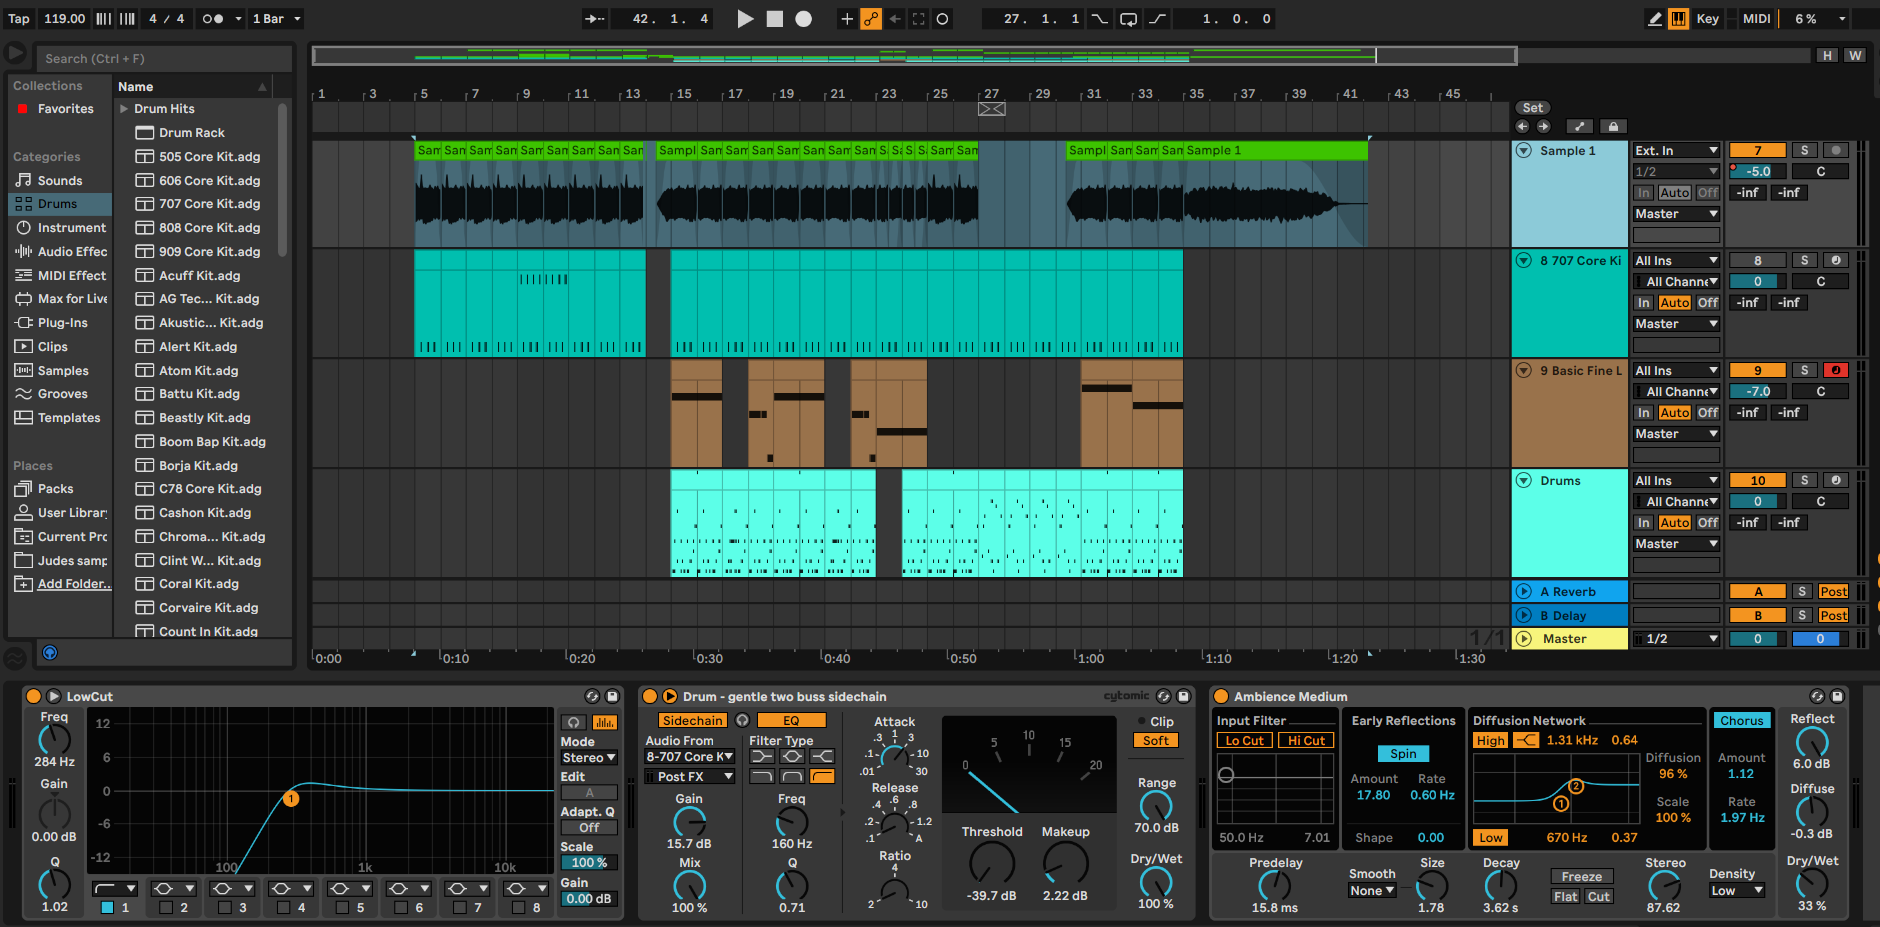
\includegraphics[scale=0.3]{images/ableton example.png}
    \caption{UI of Ableton Live}
    \label{fig:ableton}
\end{figure}

Ableton Live's main interface consists of ``tracks" which can contain either sound clips or MIDI sequences which define the pitches and timing of notes to be digitally generated. \textbf{The horizontal axis represents time}, starting at the left-most point and moving to the right. \textbf{The vertical axis generally represents different instruments (in separate tracks), and sometimes pitch}. Effects can be added to individual tracks or groups of tracks, and parameters of both the effects and track playback adjusted. 

\textbf{This structure and design is typical for DAWs}, and works with an intuition that lines up with traditional composition - each track corresponds to an instrument which can be fed through different effects. Visually, \textbf{this approach resembles modern staff notation} (see \Fref[main]{fig:staff_not}), where the horizontal axis represents time, the vertical axis represents pitch, and different instruments or parts are placed on separate staffs (collections of 5 horizontal lines).

\begin{figure}[h]
    \centering
    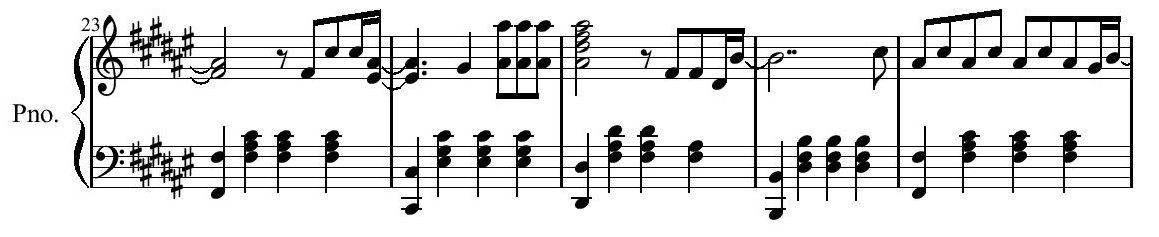
\includegraphics[scale=0.7]{images/modern staff notation.png}
    \caption{Example of modern staff notation}
    \label{fig:staff_not}
\end{figure}

This representation of audio is well established and will have been encountered by almost all musicians. This is important as users expect certain features implicitly from all designs, such as the horizontal axis representing the passage of time from left to right.

Whilst this typical representation has been refined for centuries and proven to be efficient for expressing the intentions of Western classical composers, particularly when composing for standard ensembles of instruments like orchestras, \textbf{there are many styles that are not fluently transcribed into this notation}. Pardue et al. previously analysed the issues regarding the rigidity of the design of commercial DAWs, and the limitations they have \cite{Pardue22}. This can be observed in the notation for Joshua Alvarez Mastel's composition \textit{animal}\footnote{\url{https://joshuamastel.com/animal/}}, which has an extremely complex score. This piece was given as an example by the artist involved in this project as an exemplary phonological composition.

\subsection{Live Coding}
An existing alternative to DAWs for digital composition is live coding, a technique used to generate various forms of art in real-time using a programming language. For music, a popular example is Sonic Pi.

\begin{figure}[h]
    \centering
    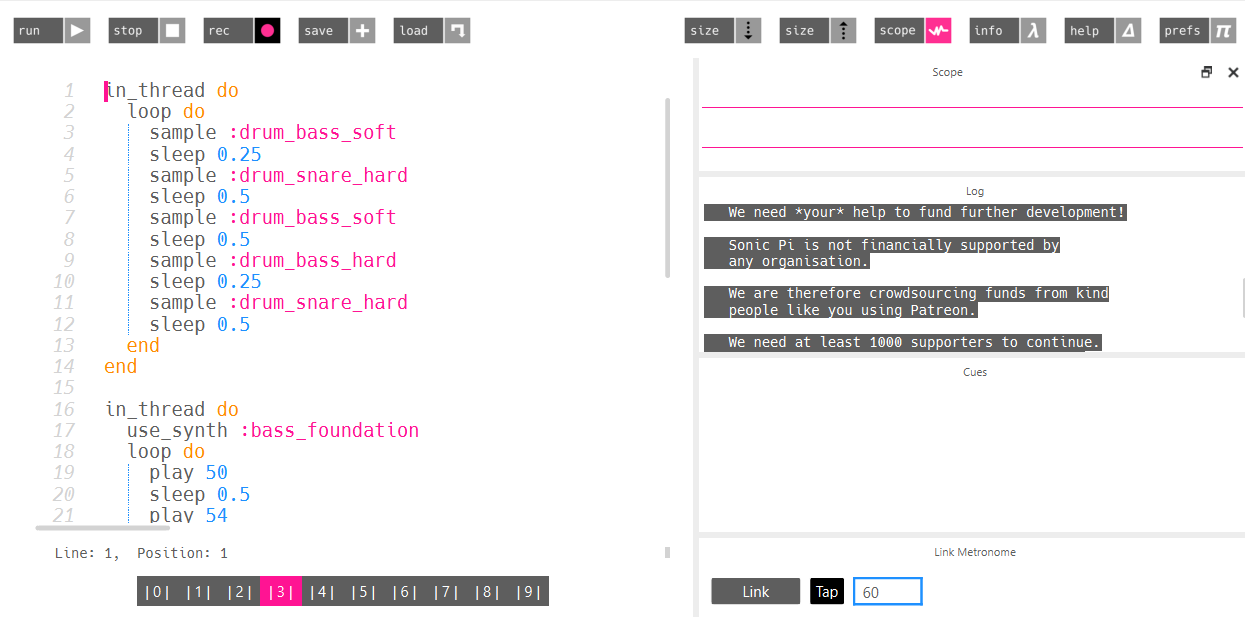
\includegraphics[scale=0.4]{images/sonicpi.png}
    \caption{UI of Sonic Pi, a popular musical live coding platform.}
    \label{fig:sonic_pi}
\end{figure}

Live coding software allows users to generate audio through writing programs, with the defining feature being \textbf{the ability to modify the code whilst the audio is running} and seamlessly change the audio as it is played. This approach to making music breaks away from the industry-standard of DAWs, and is often used for performance art, whereas DAWs are generally used for intricate, precise production of music to be listened to digitally as an exported audio file.

Live coding platforms differ from DAWs in that there is generally less complex functionality, with a focus on simpler, faster audio manipulation. The \textbf{repetition and augmentation of sounds previously defined} is the primary focus of these manipulations. This makes the process of live coding plausible in real-time whilst still sounding good. This approach is much closer to the goal of this project, and was therefore a primary focus of research and preparation.

The design of live coding platforms is integral to this project, as they focus on defining sounds and loops of sounds which are played back live, and augmented as they play. However, live coding platforms, being text-based, have no graphical interface and so they are unable to deliver accessibility to artists who are less tech-savvy. This also means that they do not provide visual notation for the music being composed. \textbf{This project is a live coding platform at its core, with a visual programming language rather than a text-based one.}

\section{Sonic Pi and Strudel}
To implement the text-based tool, an existing live coding platform was needed to build on. Sonic Pi and Strudel are two examples of such platforms and are explored here.

Sonic Pi is written in C++ and Ruby. The GUI is written in C++ whilst the code parsing and audio generation is done in Ruby. It synthesises audio by sending OSC (Open Sound Control) messages to SuperCollider, which keeps track of all synthesisers, samples and effects being triggered by the Sonic Pi interface. The codebase is large, but it does have an API, meaning that one could develop their own platform and use the Ruby portion of the software to generate sound using SuperCollider easily without the C++ GUI.

Strudel is a web-based live coding platform built in JavaScript, based on another live coding language called TidalCycles. It mainly uses the Web Audio through a framework called Tone.js to synthesise audio, and was still in an experimental stage of development at the time of this project being researched. The software is relatively small, and the codebase easy to navigate and manipulate, as it is written in a modular style that splits up different parts of the software into separate packages which can be used individually.

The text-based tool in my project built upon the Sonic Pi platform, as it has the functionality to fully support its development.

\section{Speech synthesis}
A desirable feature would be to include a way of generating phonological sounds digitally, to allow the user to utilise and manipulate speech sounds without recording and re-recording themselves speaking. However, digital speech synthesis is an extremely difficult task and was ruled to be out of scope for this project \cite{Balyan13}. I experimented with vowel synthesis - a fundamental subset of speech synthesis - during the first stage of the implementation. This is detailed in \Fref[main]{sec:vowel_synth}.

\section{Software Engineering}
This section outlines some of the research that went into the specifics of the project's implementation, and the choices that were made prior to streamline the development process.

\subsection{Related work}
This project builds upon work in a large field of research concerning the development of novel expressions for digital music. Of particular relation to my project is the International Conference on New Interfaces for Musical Expression (NIME), which has been held annually for the past 21 years, presenting the latest work in new musical interface design, with a focus on human-computer interaction and computer music \cite{NIME}.

One related piece of work is an exploration by Dal R{\` i} et al. into the generation of visual scores to accommodate live coding practices \cite{Dal22}. Their work attempts to introduce a tool for visualising live coding pieces, to provide a sort of score that represents the piece.

\subsection{Framework}
As mentioned, Sonic Pi was used to develop the text tool as it provided the necessary features for its demonstrative purposes.

For the graphical interface, I needed a platform that has the functionality to support my development, and that is malleable enough to accurately represent the design of the tool; I needed a platform that is capable of either generating high-fidelity audio or fluently using another system to do so.

Electron is a JavaScript framework which builds desktop applications using Chromium, rendering a web-page in a native window. It uses Node.js as the JavaScript. Node.js provides extra functionality and enables the use of essentially any JavaScript library, through the npm package manager. Electron is a popular, well-documented framework, which is beneficial in a project with little development time. It powers applications like Discord, Skype, Twitch and Notion.

\subsection{Libraries}
\subsubsection{Audio}
Tone.js is a Web Audio framework which supplies an API for audio applications written in JavaScript. It supplies reliable event scheduling, audio playback from files, and a system for linking effects and sounds together, and through to output. The features supplied by this library fully support this project, providing the functionality need for timekeeping, audio playback and audio effects. It is used in Strudel for audio generation. Due to its flexibility, full documentation, and widespread usage, this library is used in my project.

\subsubsection{Visual Interface}
p5.js is a JavaScript library which provides basic graphical capabilities, with a co-ordinate system. p5 has no strict structure, supplying the developer with a canvas that can be drawn onto however they need. This allows the developer to have full control over what is rendered in the application. Because of this fluidity, p5 is used to render the visual interface.

\subsection{Programming Languages}
The text tool was written in the Sonic Pi GUI, in Sonic Pi's own language, which is an extension of the Ruby programming language.

The final project is written in TypeScript, an extension of the JavaScript language which allows static type-checking, and transpiles into JavaScript code. It also adds a few features that provide better support for object-oriented programming, which was deemed valuable to this project, as explained in \Fref[main]{sec:comp_rep}. Classes are extremely limited in JavaScript as it is dynamically typed. TypeScript allows for typing members, variables, and parameters, which prevents many bugs as obvious type errors will be avoided. This also makes the debugging process more straightforward, as one can analyse the types of different variables.

\subsection{Development Methodology}
It is important to approach software development with a solid plan dictating logical, reasonably sized steps from beginning to conclusion. As shown in the project proposal (\Fref[main]{appendix:proposal}), the project was planned out in fortnightly blocks in order to ensure that each stage of the project was carried out in a timely manner. Due to the experimental nature of this project, it was impossible to know exactly how the implementation would go from start to finish, and so it took part in two stages. 

The first stage consisted of the development of the text-based tool and the computational model of composition. These aspects of the project were developed iteratively, taking advantage of the ease of implementation in Sonic Pi to supply the artist involved with regular updates, getting feedback on what is useful for the artist and what isn't as necessary and wouldn't be a priority in the graphical tool. This would refine the idea of what is crucial to the structure of phonological composition being represented in a graphical interface.

The second stage consisted of the development of the graphical tool, which suits the waterfall development methodology. At this stage, the graphical tool would be fully planned out and designed, and so the development could be broken down into the implementation of individual features, with essential prerequisites like playback of audio being fully implemented before features that need others to be implemented, like audio effects.

\subsection{Tools}
For the development of the text-based tool, I simply used Sonic Pi's GUI to write code.

For the graphical tool, I used Visual Studio Code as an IDE. VS Code was an obvious choice, as it is powerful and very customisable. There exists many community-made extensions which can enable one to use various tools easily in your code, such as TypeScript. It also has a built-in Git tool which made for easy version control and backing up.

I used GitHub to back up my repository and Git for version control. As stated, this was easy to do with VS Code. This minimised the risk of data loss, as even if my laptop was lost or destroyed, I could retrieve my work. In the same vein, I wrote all of my notes during the project in Notion which automatically backs everything up to the cloud.

\chapter{Implementation}
This chapter outlines first the development of the text-based tool and computational model of composition, followed by the design and implementation of the final graphical composition system.

\section{Text-based tool}
As described in the preparation, it was decided that Sonic Pi would be used for the implementation of the text-based tool, using it to experiment with possible features that would benefit phonological composition, and to get feedback from the artist. This section describes the general structure of phonological compositions as well as the design of this text-based tool.

\subsection{Phonological composition structure}\label{sec:phonology}
\textit{Note: for simplicity, I will only discuss English in the section. Much of the analysis applies directly to most other languages, but certain concepts such as morphemes and syllables are subtly different around the world.}

In order to develop the text-based tool, it is important to first understand what features the compositions may incorporate and so an understanding of phonological structures is vital. In linguistics, it is common to represent language as a tree, with individual words as leaf nodes. These trees are referred to as \textbf{parse trees}.
\begin{figure}[h]
    \centering
    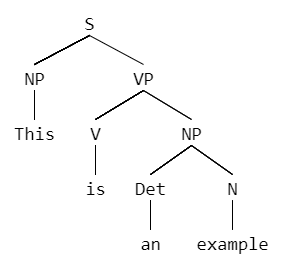
\includegraphics[scale=0.5]{images/parse_tree.png}
    \caption{An example of a constituency-based parse tree.}
    \label{fig:parse_tree}
\end{figure}

The tree structure is used as it accurately represents the structure of many written natural (as well as formal) languages, like English. A key feature of the tree structure is the idea of recursion; a node in a tree can contain nodes with the same structure as itself, continuing on indefinitely\footnote{Interestingly, in an article from 2002, N. Chomsky et al. \cite{Hauser02} argue that recursion is the singular feature that distinguishes the human faculty of language from other animals }. In these trees, words are the smallest possible units of language, but in alphabetic languages, words are made of \textbf{morphemes}, which in turn consist of one or more letters. This idea of breaking up sentences, phrases and words into smaller pieces is of particular interest for phonological composition, as seen in \Fref[main]{sec:art_background}.

\textbf{This analysis motivates the necessity for a recursive structure in the design of the tools.} There needs to be a concept of elements containing smaller elements which could contain smaller elements still, until we get down to the atomic elements, individual spoken sounds.

In spoken language, this structure persists still, but words are represented through sounds rather than shapes. These sounds can be characterised as individual syllables, or in writing through phonetic notation, such as the \textbf{International Phonetic Alphabet} (IPA), which was of interest for this project.
\begin{figure}[h]
    \centering
    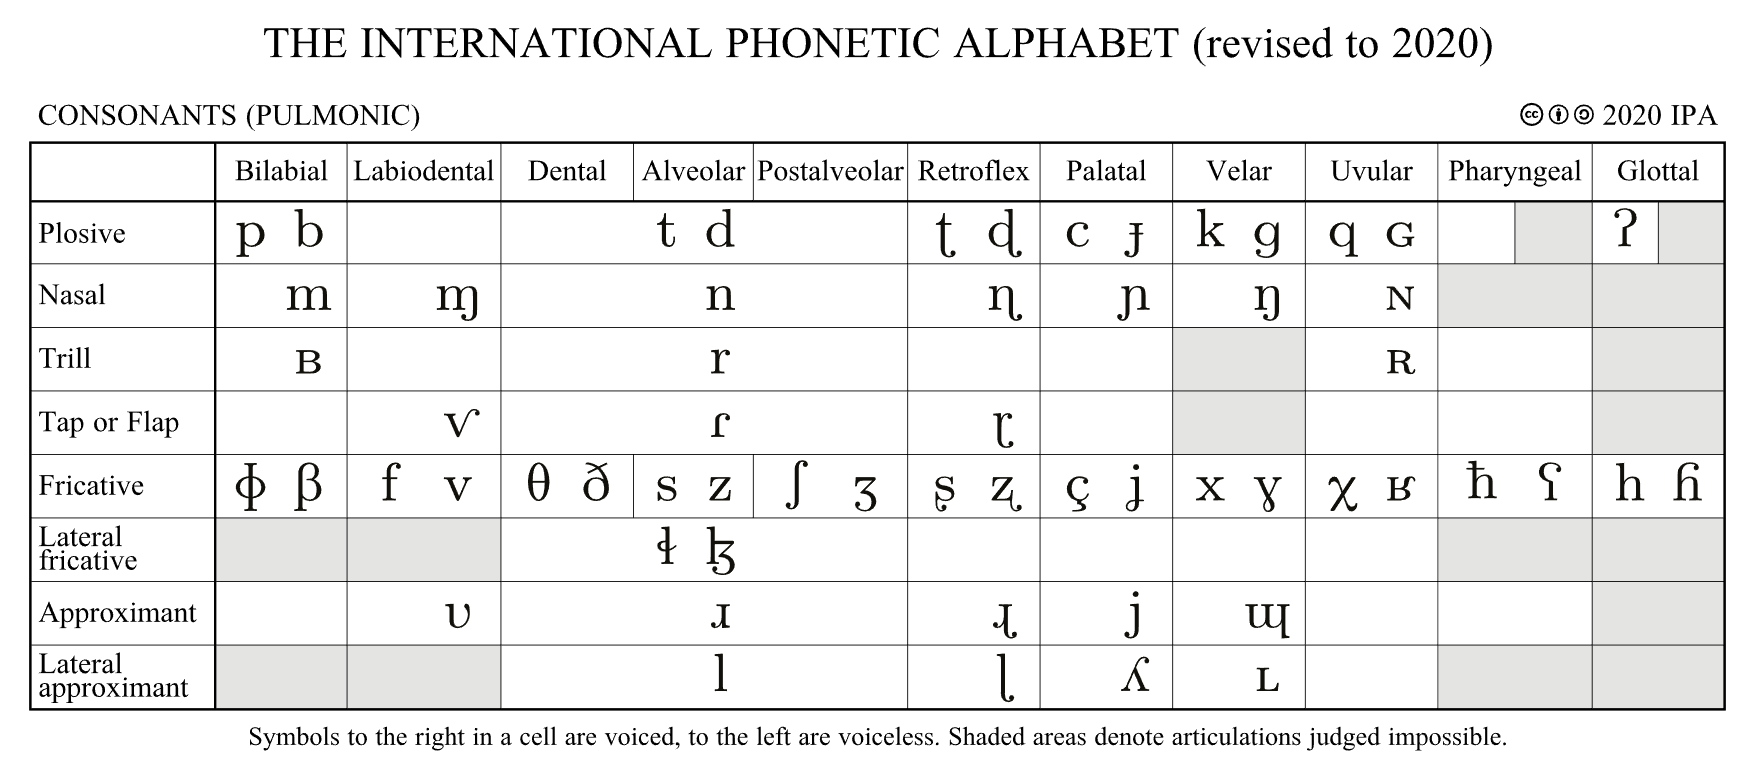
\includegraphics[scale=0.3]{images/IPA.png}
    \caption{A portion of the official IPA chart.\protect\footnotemark}
    \label{fig:ipa_chart}
\end{figure}
\footnotetext{Image from International Phonetic Association, under the CC BY-SA 3.0 license: \url{https://creativecommons.org/licenses/by-sa/3.0/deed.en}, cropped by myself}

An idea to extend the text tool's functionality was to represent sounds by characters from the International Phonetic Alphabet, as they cover almost all sounds used in human spoken language. Characters in the IPA represent vocal sounds or modifications to vocal sounds which have a lexical impact on what is being said. That is, if you were to replace one sound or modification with another, the meaning of the word being said may change. It was discovered during research that there is no problem using IPA characters in Sonic Pi, and they can be used in strings and even as function and variable names.

The letters in IPA represent consonant or vowel sounds, which can then be modified by diacritics. For example, the character b represents the first sound in the English word ``bit", and we can attach a diacritic to have it read in ``breathy voiced" form: \textsubumlaut{b}.

With this in mind, we have two elements for the design: the narrative structure of the composition, which relates to the linguistic tree structure, and the actual sounds and modifications to sounds being made.

\subsection{Vowel synthesis}\label{sec:vowel_synth}
Digital speech synthesis in general is a difficult problem with a rich history. Modern solutions are impractical for the purpose of this project. Vowel sounds can be synthesised to an adequate level by using formant synthesis, where a bandpass filter is applied to a sawtooth signal. I decided to experiment with this type of synthesis during the creation of the text-based tool as these features are present in Sonic Pi. However, the resulting sound is very robotic can not be altered by any parameters in an intuitive way, and I determined that this feature would not make a meaningful contribution to my project.

\subsection{Computational representation}\label{sec:comp_rep}
In order to represent the compositional structure, it is essential to organise sounds recursively. A user should be able to define a word as a collection of syllables, or a line as a collection of words. There are a number of ways to achieve this computationally.

A natural approach is object-oriented programming. Defining a class which could either contain a sound clip or a collection of objects with the same type supplies all the capability needed to represent the aforementioned phonological tree structure. Objects which simply contain a sound clip are leaf nodes in the tree, and objects containing collections of other sound objects are the parent nodes. These nodes could have names denoting what structure they represent, such as a syllable, word, or sentence.

\begin{figure}[h!]
    \centering
    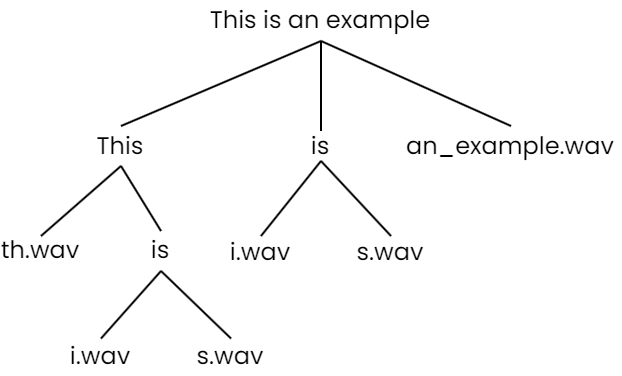
\includegraphics[scale=0.5]{images/tree_structure_example.png}
    \caption{Example of a possible tree built with the text tool's computational representation.}
    \label{fig:tree_struct_ex}
\end{figure}

Unfortunately, Sonic Pi does not allow for classes to be created, so this approach does not apply for the text tool, but the concepts of the approach can still be applied. Instead of dedicating a class to define this type of object, we instead use lists which contain lists or sound files.

It is still desirable to have the ability to change some parameters associated with the sounds, though, even without being able to define a class which would have these parameters as its local members. For this, we store the sound files as a tuple, containing a file name referring to a sound file to be played, along with one or two parameters.

\subsection{Final text-based tool}
The final implementation of the text-based tool consists of a collection of functions which can:
\begin{itemize}
    \item Create lists of sounds.
    \item Translate a string of IPA characters into a list of file names storing the sounds they represented.
    \item Take a list containing sounds, or other lists, and play them back with the appropriate timing.
    \item Reverse a list of sounds (in a deep sense, each list contained in the list would also be reversed).
    \item Set all sounds in a list to last the same duration.
\end{itemize}

Sounds are represented by a tuple:
\begin{equation*}
    \{sample,\ length,\ gap\}
\end{equation*}

\begin{description}
    \item[sample] - Stores a string referring to a file name, to be played.

    \item[length] - The amount of time the sample should play for, relative to how long the sample is. The sample is stretched such that it is played for $sample\_duration * length$ seconds.

    \item[gap] - The amount of time after the sound plays that the next sound should start, relative to the duration of the sample. After playing this sound, the program waits $sample\_duration * length * (1 + gap)$ seconds before playing the next sound. If this value is negative, the next sound will overlap with the current sound, which can make for more realistic speech when using individual consonant/vowel sounds.
\end{description}
\newpage
\section{tuPAC}

This section describes the culmination of all previous work described in this dissertation, the design and implementation of the \textbf{Totally Usable Phonological Audio Composer}, or tuPAC for short.

\subsection{Visualising compositional structure}
When designing the graphical interface, it was vital to have an accurate visual representation of phonological composition, in order for the user to easily create and manipulate them whilst using it. There needs to be a clear representation of individual sounds, and the components containing those sounds. Existing software designs can provide context and inspiration, and thus are analysed here.

\subsubsection{Scratch}
Scratch is a very popular visual programming language that is commonly used to introduce children to the ideas behind programming without the difficulty of writing code in text form, which can be intimidating at first. This platform is of relevance to my project due to its similarity in motivation to my program: making a visual interface to improve accessibility to a task which is typically complex and technically done digitally. 

Scratch uses blocks to represent events in either the project or the control flow of the events. These blocks are dragged over from a menu and arranged however the user desires on a blank surface.

\subsubsection{Field}
A major source of inspiration for the program's final interface was Field, which is a live coding software made by OpenEndedGroup\footnote{Github repository of Field: \url{https://github.com/OpenEndedGroup/Field2}} not for music, but for visual art. Field allows users to generate moving digital art, and the live coding background means that this design is very relevant to my own project. The interface consists of a canvas which can contain boxes, which can have code written to be associated with them. A line marking the current ``time" runs over the screen, executing code in boxes as the line runs over them. The code can use the current position of the line as a parameter, and is used to generate visuals. 

\newpage
\subsection{Final Design}\label{sec:final_design}
\begin{figure}[h]
    \centering
    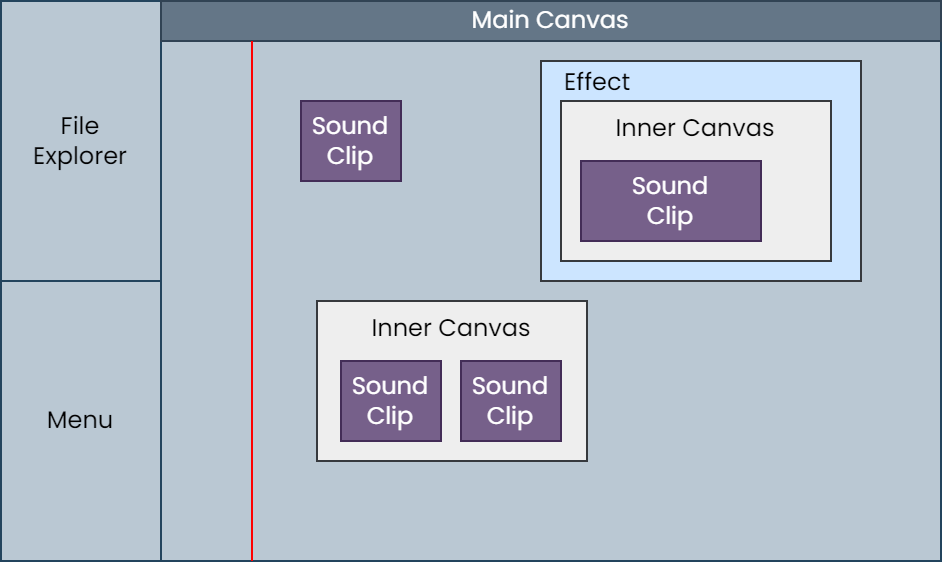
\includegraphics[scale=0.4]{images/final_design.png}
    \caption{An example of what the final design would look like during use. Nested boxes correlate to the tree structure of composition.}
    \label{fig:final_design}
\end{figure}

The final design incorporates ideas from Field and Scratch and creates a visual representation of the phonological composition structure. The interface consists of a main canvas, an element menu, and a file menu. The canvas is much like the canvas in Field, with a line moving from left to right, activating boxes representing sounds as it passes over them. In order to represent the recursive type of the canvas, we have the boxes in the canvas to be either a sample linked to a sound file, or another canvas, with all of the capabilities of the main canvas. Similarly, effects are boxes which can contain smaller boxes, to which that effect will be applied. Like Scratch, a side menu is available to drag-and-drop new elements - samples, canvases or effects - onto the canvas. This is a highly legible way of demonstrating to users what they are able to do in tuPAC.

This design was the final step before the implementation of the graphical tool. Next, we look at how the tool works.

\subsection{Program structure}
\Fref[main]{fig:tupac_structure} gives an overview of the general structure of the software at runtime. The \verb|main.js| file is run first, which imports Electron, containing Node.js and Chromium. It creates a window with the layout described by \verb|index.html|. On loading the webpage, \verb|tupac.js| is run, creating a p5.js canvas on the page. The p5.js library runs the setup function once and then repeatedly runs the draw function, rendering the GUI of tuPAC. These functions are defined in \verb|tupac.js|.

\begin{figure}[h]
    \centering
    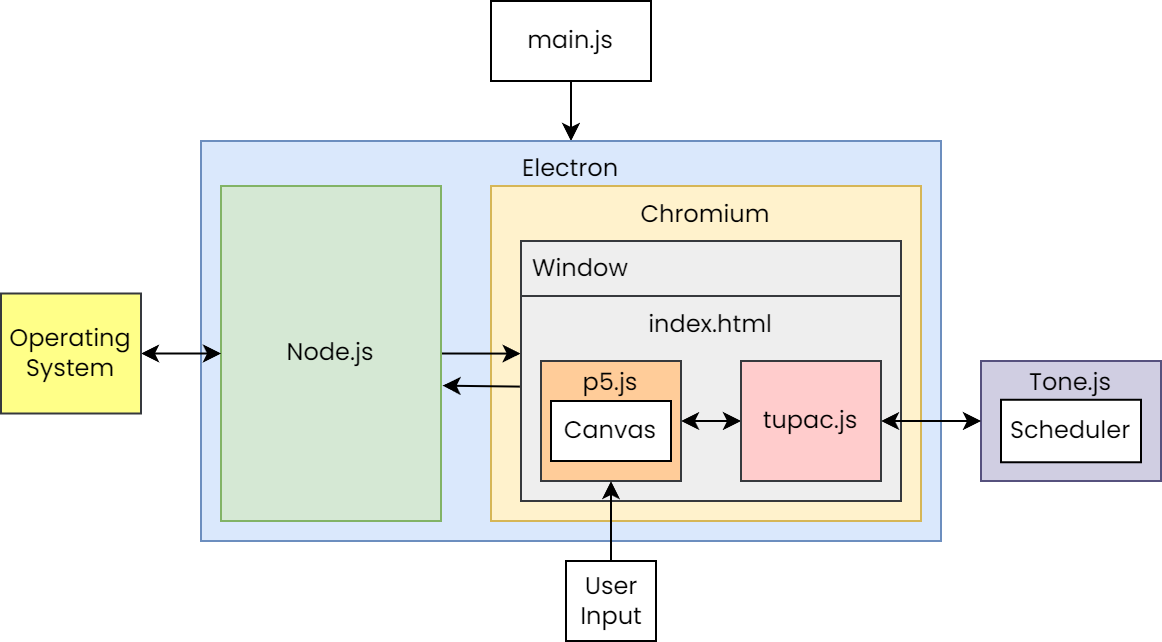
\includegraphics[scale=0.35]{images/tuPAC_structure.png}
    \caption{The high-level runtime structure of tuPAC. Arrows indicate some form of communication between components.}
    \label{fig:tupac_structure}
\end{figure}

As mentioned previously, TypeScript was used to facilitate the usage of the object-oriented programming paradigm. The nature of object-oriented programming allows for a relatively simple translation of the design of this program into a computational model, as discussed in \Fref[main]{sec:comp_rep}. We want the ability to instantiate objects of a certain type, and pass objects around knowing they will have certain methods, which isn't possible in vanilla JavaScript as it is dynamically typed. In the \verb|/src/| directory, each file (besides \verb|tupac.js|) contains one or two classes, which are imported by other files and used during runtime to represent each part of the program.

When the setup function in \verb|tupac.js| is run, it instantiates a \window\ object, and populates it with the two side menus and a main canvas, as shown in \Fref[main]{fig:final_design}. The rest of the program then relies on user input.

\subsection{Elements}
In tuPAC, everything that is rendered on the screen is an \element, i.e. every class that will be rendered extends the abstract \element\ class. The \element\ class defines the members and methods that everything in the program needs to have, and provides default versions for them.
\begin{table}[h]
    \centering
    \begin{tabular}{c|c|p{300pt}}
        Name & Type & Description \\
        \hline
        pos & \pos & The co-ordinates of the top-left corner of the \element\\
        size & \pos & The size of the \element\\
        minSize & \pos & The minimum size to allow when resizing\\
        draggable & \verb|boolean| & Whether this \element\ can be moved by the user\\ 
        resizable & \verb|Resi| & Whether this \element\ can be resized, in each direction\\
        parent & \element & The \element\ which contains this one. If this \element\ is on the top level, then this is \verb|null|\\
    \end{tabular}
    \caption{The members defined in the abstract \element\ class}
    \label{tab:element_members}
\end{table}

In \Fref[main]{tab:element_members}, \verb|Resi| refers to an Enum\footnote{\url{https://www.typescriptlang.org/docs/handbook/enums.html}} which can be to any of the values in the set \{None, X, Y, XY\}, indicating whether or not the \element\ can be resized by the user in the X and Y directions. The \pos\ class is described in \Fref[main]{sec:pos}.

\begin{figure}[h]
    \centering
    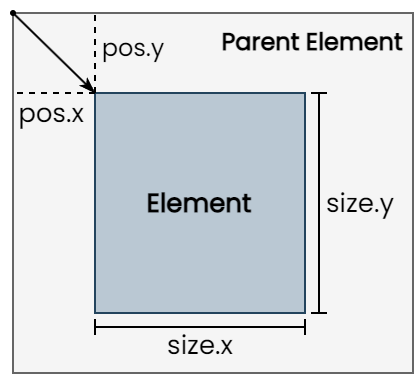
\includegraphics[scale=0.6]{images/element_demonstration.png}
    \caption{The meaning of the size and pos members of \element. If an \element\ has no parent, this refers to the application's window.}
    \label{fig:element_demo}
\end{figure}

The \element\ class supplies a number of methods which are useful for all \element s to have, or can be overridden by subclasses. Two methods are left abstract, meaning that subclasses need to have an implementation in their definitions. These methods are \verb|draw| and \verb|clicked| and are called when the \element\ should be drawn onto the screen and when a user clicks on it, respectively.

Note that the p5.js library uses the top-left corner as the origin of co-ordinates, meaning that the \verb|x| co-ordinate indicates the distance from the left-hand side of the window, and the \verb|y| co-ordinate indicates the distance from the top of the window. In tuPAC, this convention is maintained.

\subsection{Instrumental Classes}
\subsubsection{Pos \& Box}\label{sec:pos}
Being a graphical software, tuPAC makes frequent use of co-ordinates and pairs of co-ordinates. The classes \pos\ and \boxT\ help with the handling of these by wrapping them up into single objects and providing methods to easily manipulate them.

\pos\ objects have two members: x and y. The class provides methods such as adding co-ordinates together, multiplication by a scalar and finding the piece-wise minimum of two \pos\ objects.

\boxT\ objects have two members: origin and size. These members are both \pos\ objects specifying the position of the top-left corner and the size of a box, respectively. This class supplies methods to utilise \boxT s, like checking whether a co-ordinate is in a \boxT\ and moving a \boxT's origin such that it sits inside a larger \boxT.

\subsubsection{Control Bar}
Many of the \element s in tuPAC have bars along the top which can be used to drag them, can have buttons which control the \element, and can have text to describe them. These are referred to as \controlbar s, the name of the class which defines these objects.

\subsubsection{Playable}
\playable\ is an interface that specifies \element s that can be played. It ensures that all \playable\ \element s have methods for playing, pausing, stopping and scheduling playback.

\begin{figure}[h]
    \centering
    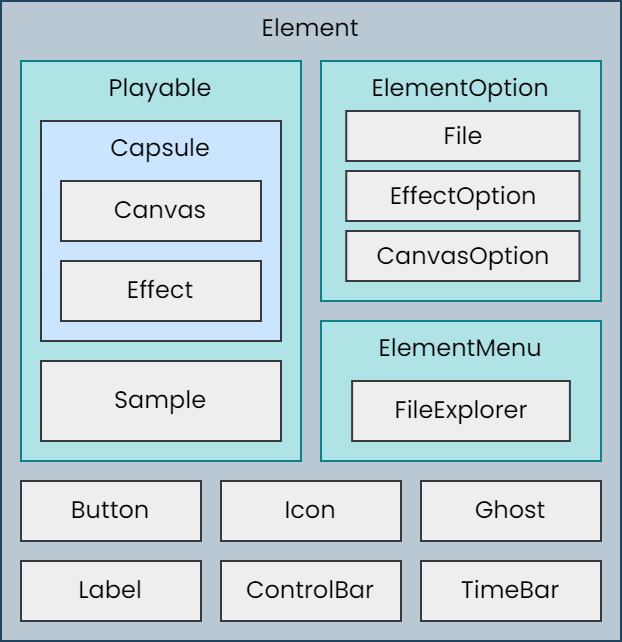
\includegraphics[scale=0.4]{images/tupac_class_structure.png}
    \caption{The inheritance structure of all classes that extend \element. All smaller boxes contained in larger boxes are subclasses of the larger box.}
    \label{fig:element_inheritance}
\end{figure}

\subsection{Canvas}\label{sec:canvas}
The most important \element\ in tuPAC is the \canvas. When the program first starts, the user is presented with a blank \canvas\ object, alongside the menus. This class represents the nodes of the phonological tree structure as described in \Fref[main]{sec:comp_rep}. They represent a sound or a collection of sounds; when a \canvas\ plays, its \timebar\ moves from left to right, and any sounds underneath the bar get played.

\begin{figure}[h]
    \centering
    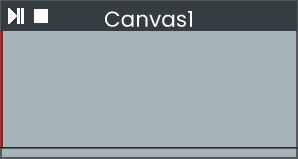
\includegraphics{images/canvas.png}
    \caption{An example of a \canvas.}
    \label{fig:canvas}
\end{figure}
\newpage
\canvas\ objects visually consist of:
\begin{itemize}
    \item A \controlbar\ with a title, play/pause button and stop button. The play/pause button starts the \canvas\ playback if it is paused, and pauses the \timebar\ where it is if not. The stop button stops the playback and moves the \timebar\ back to the start of the canvas. The title can be clicked on and written into, to name the \canvas\ however the user likes.
    \item A blank space which can hold any other \playable s to be played when the \canvas\ plays.
    \item A \timebar\ which scrolls from left to right across the \canvas, playing any \element s inside the \canvas.
    \item A box which translates the \timebar\ inside the \canvas\ to the \canvas' parent. This does not exist on the main \canvas, as it has no parent. This is explained in \Fref[main]{sec:timebar_translate}.
\end{itemize}

\subsection{Samples}
The \sample\ class is where all audio in tuPAC originates. These \element s represent an audio file to be played as a \timebar\ scrolls over them.

\subsubsection{Waveforms}
\sample s are drawn as a ``waveform overview", meaning that they are visually represented by an approximate chart of the amplitude of the sound wave over time. For audio clips, this is perceived as the volume of the sound over time. This representation helps to distinguish one clip from another, as well as allowing users to see if there are periods of silence in the audio before playing it. This is also a standard representation in audio software, so users may expect this to be what audio looks like. It is helpful to use existing notation, which users will have likely encountered before, for the \clarity\ of the visual representation.

The amplitude of a wave has various definitions. Here, we are considering the volume of an audio clip over time, and so it is defined as the maximum absolute value of the signal. We approximate the transient amplitude of an audio clip by using the maximum magnitude within a range at different points throughout the clip. As audio files are discrete rather than continuous, this can simply be defined as the greatest absolute value in a given range, as shown in \Fref[main]{fig:amplitude}. When discussing audio files, I will refer to the individual magnitude values as samples, as is standard in audio processing. This should not be confused with the class, which is written as \sample.

\begin{figure}[h]
    \centering
    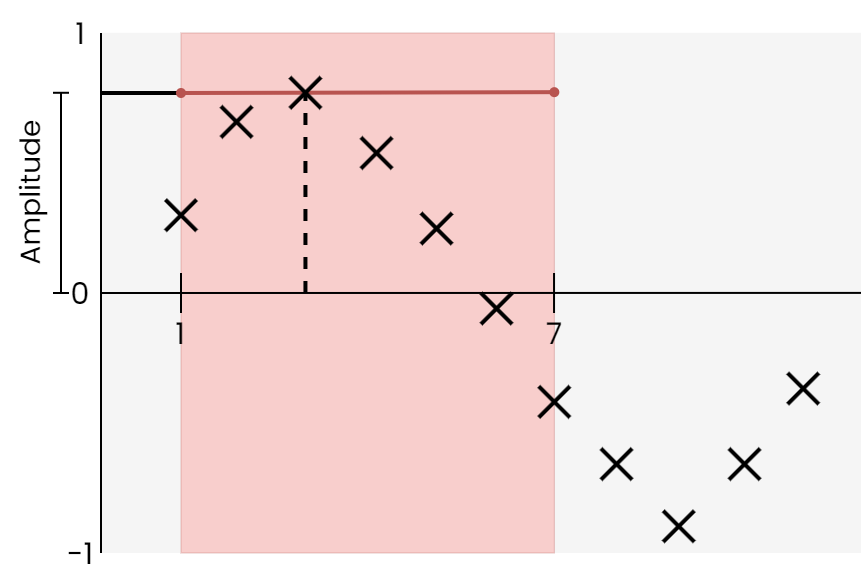
\includegraphics[scale=0.3]{images/amplitude_example.png}
    \caption{This diagram illustrates how we obtain the amplitude of an audio clip within a given range. Here the range is [1,7] and the sample with the highest absolute magnitude is the 3rd.}
    \label{fig:amplitude}
\end{figure}

In order to generate a waveform overview, the audio first needs to be split into a set of ranges and then the amplitude of each range found. In tuPAC, this is done with \Fref[main]{alg:waveform}. For a given bounding box, this algorithm generates an array of bar heights corresponding to a given audio file. This waveform can then be drawn as a collection of vertical lines in the \sample's \verb|draw| function.

\begin{figure}[h]
    \centering
    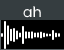
\includegraphics[scale=1.5]{images/sample.png}
    \caption{Example of a waveform drawn on a \sample.}
    \label{fig:my_label}
\end{figure}

In tuPAC, the audio generation is done with Tone.js. After loading a sound file to be played in a \sample\ we can acquire an array for floating point numbers between $-1$ and 1 representing the magnitude of each sample in the audio file. We can then run \Fref[main]{alg:waveform} on this array to get an array of bar heights.

When generating a waveform, we generate an array with arbitrary size from an array with arbitrary size. Thus, we must ensure that no matter what size each array is we will get a waveform that approximately represents the audio.

\begin{algorithm}[H]
\DontPrintSemicolon
\SetKwInput{Input}{Input}\SetKwInOut{Data}{Constants}
\Input{\textit{WaveformLength}: In pixels, the horizontal length of the waveform.
\newline
\textit{WaveformHeight}: In pixels, the maximum vertical height of bars in the waveform.
\newline
\textit{ArrayOfSamples}: The buffer from Tone.js, arbitrarily large.}
\Data{\textit{BarThickness}: In pixels, the thickness of each bar when drawn.
\newline
\textit{BarPad}: In pixels, the distance between bars when drawn.
\newline
\textit{MaxWidth}: In samples, the maximum size of the range to get amplitude from.}
\vspace{1mm} \hrule \vspace{1mm}
\nl $NumberOfBars \gets WaveformLength/(BarThickness + BarPad)$\;
\nl $Waveform \gets []$\;
\nl $Ratio \gets ArrayOfSamples.length / NumberOfBars$\;
\nl $Width \gets \lfloor min(MaxWidth, ratio)/2\rfloor$\;
\nl \For{$i=0$ to $bars-1$}{
    \nl $Centre \gets i * Ratio$\;
    \nl $Range \gets [Centre-Width, Centre+Width]$\;
    \nl $Waveform[i] \gets max_{j\in Range}(|ArrayOfSamples[j]|)$\;
}
\nl $MaxValue \gets max_{n\in Waveform}(n)$\;
\nl \For{$i=0$ to $bars-1$}{
    \nl $Waveform[i] \gets WaveformHeight * Waveform[i] / Max$\;
}
\caption{tuPAC waveform generation algorithm}\label{alg:waveform}
\end{algorithm}

\begin{figure}[h]
\centering
\begin{subfigure}{.5\textwidth}
  \centering
  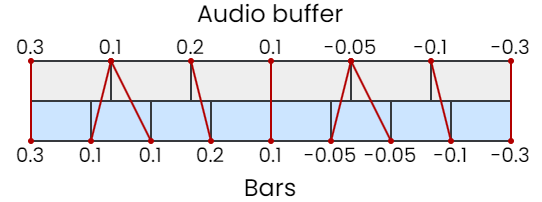
\includegraphics[width=\linewidth]{images/waveform_range_diagram_a.png}
  \caption{$\frac{s}{b} \approx 1$}
  \label{fig:waveform_range_a}
\end{subfigure}%
\begin{subfigure}{.5\textwidth}
  \centering
  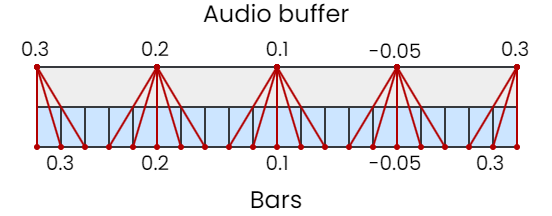
\includegraphics[width=\linewidth]{images/waveform_range_diagram_b.png}
  \caption{$\frac{s}{b} \ll 1$}
  \label{fig:waveform_range_b}
\end{subfigure}\\[1ex]
\begin{subfigure}{\textwidth}
  \centering
  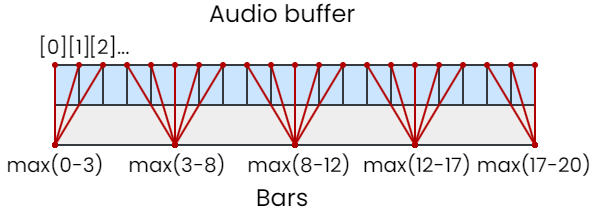
\includegraphics[width=.6\linewidth]{images/waveform_range_diagram_c.png}
  \caption{$\frac{s}{b} \gg 1$}
  \label{fig:waveform_range_c}
\end{subfigure}
\caption{These figures illustrate the desired behaviour for part of \Fref[main]{alg:waveform}, in 3 characterizations of the problem. $s$ denotes the number of samples in the audio buffer array, $b$ represents the desired number of bars in the waveform. In the algorithm, this behaviour is achieved by taking the maximum across a range of samples, with the range being of size 1 if $\frac{s}{b}\le 2$.}
\label{fig:waveform_range}
\end{figure}

As illustrated by \Fref[main]{fig:waveform_range}, \Fref[main]{alg:waveform} aims to map values of the audio buffer to the bars. It then normalises the values to be displayed such that the largest bar is as tall as the desired waveform height. The values are mapped by multiplying the index of the bar by $ratio = \frac{samples}{bars}$. This will give us a value in the range $[0,samples]$, to access the audio array with. We also use $ratio$ to calculate how large of a range to access in the samples for each bar. This is due to the definition of amplitude stated earlier. The amplitude to be represented by each bar will be a better approximation if the maximum absolute value within a range is taken rather than just the value of the closest value.

\subsection{Time Bar Translation - \normalfont\textbf{\textsc{Extension}}}\label{sec:timebar_translate}
One important feature of tuPAC is allowing \canvas es to run at different speeds. However, this results in \timebar s moving at different speeds, which could be visually confusing and difficult to understand for the user. To solve this, there is a space in which the \timebar\ of a child \canvas\ has a line connecting it to the parent \canvas's \timebar, as shown in \Fref[main]{fig:timebartranslation}. \timebar\ translation was devised as an extension to the original core features of the project, as it contributes significantly to the intuition of users (as shown in \Fref[main]{sec:qual_res}).


\begin{figure}[h!]
    \centering
    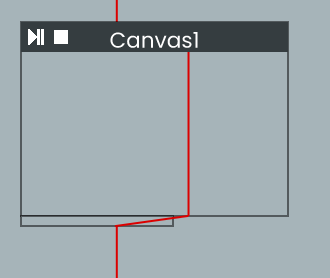
\includegraphics{images/timebartranslate.png}
    \caption{Example of a \timebar\ being ``translated".}
    \label{fig:timebartranslation}
\end{figure}

This feature acts as a visual aid for users, providing intuition for the \canvas\ structure, but it also serves a functional purpose. Naturally, as this box translates between the speeds of the two \canvas es, its horizontal size represents the duration of the child \canvas, at the parent \canvas' speed. When resized, the child \canvas' speed changes to represent the box's size. This means that the child \canvas\ plays exactly for the amount of time the parent's \timebar\ is touching this translation box. When a user resizes the time bar translation box, the speed of the child \canvas\ must be calculated and adjusted appropriately, preventing the resizing if the speed reaches a maximum of minimum. The speed of any children must also be adjusted, such that \sample s and \canvas es inside the affected \canvas\ play back at the correct speed. 

\subsection{Effects}
The \effect\ class provides a way of applying distortion or reverb to the sounds in tuPAC. As shown in \Fref[main]{fig:element_inheritance}, it extends the same class as \canvas, allowing for other \playable s to be held by an \effect. \effect s, however, can only hold one \element, this is demonstrated in the video submitted with the source code of this project. As explained in detail in \Fref[main]{sec:playback}, \effect s have a ToneAudioNode associated with them which apply the appropriate effect to signals passing through them.

\subsection{Tree Structure Realised}
By allowing a \canvas\ object to have other \canvas es in it, we implicitly create the tree structure of composition, as mentioned in \Fref[main]{sec:canvas}. When an artist creates a composition in tuPAC, they create a tree structure, with \sample s as leaf nodes, and \canvas es and \effect s as parent nodes. This fact is illustrated in \Fref[main]{fig:canvas_tree}.
\footnotetext{This tree could compositionally be understood as two trees, one containing ``the bad are" and one containing ``anybody", with two separate voices performing them, like separate staffs on sheet music.}

\begin{figure}[h!]
    \centering
    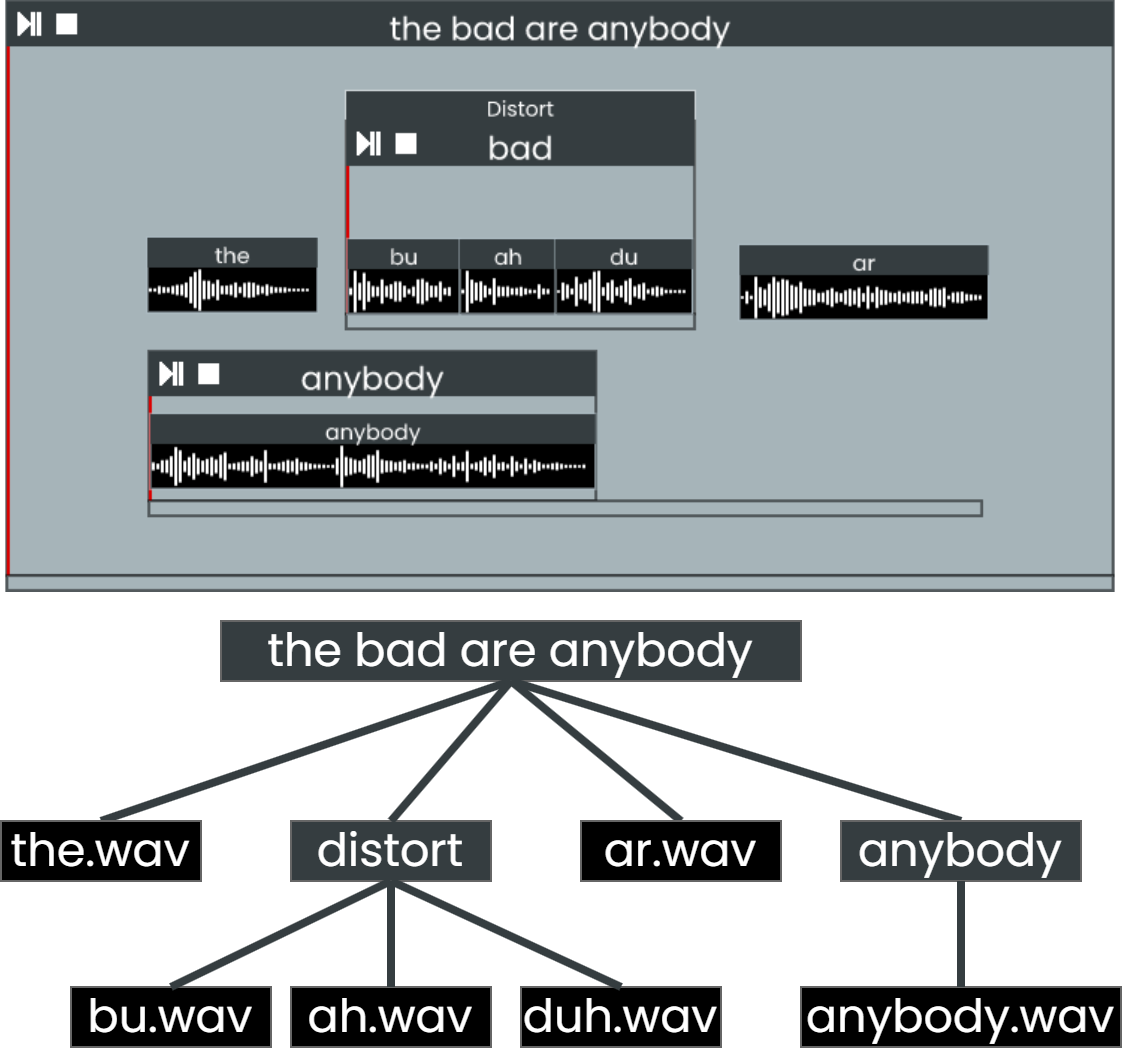
\includegraphics[scale=0.3]{images/canvas_tree.png}
    \caption{Example of a ``tree" of \playable s in tuPAC taken from one of the evaluation tasks and an illustration of that tree, with the object associated with each node containing a reference to the parent of that node. Note that here, sibling nodes can play simultaneously, so this tree is not quite like the phonological trees seen in \Fref[main]{sec:phonology}\protect\footnotemark[4]. }
    \label{fig:canvas_tree}
\end{figure}

\subsection{Rendering}
In order to facilitate the recursive nature of the \canvas\ class, the rendering of \element s is done relatively at each depth of the \canvas\ tree. The pos member of \element s are stored as co-ordinates relative to the top-left of where their parent is on the screen. This means that when moving \element s around, we do not need to translate the co-ordinates of any child \element s, as they will always be rendered relative to their parent's co-ordinates. This saves a lot of computation when users interact with the software. Because of this, the \verb|draw| command takes a parameter offset, of type \pos, which stores the absolute co-ordinates (relative to the application window) of the \element's parent. Inside \verb|draw|, the offset parameter is added to the \element's pos member. It then uses this new co-ordinate to draw itself onto the screen using p5's API and, with the new co-ordinate, calls the \verb|draw| method of any child \element s it has, such as \timebar s, \controlbar s, or indeed \playable s.

\begin{algorithm}
\DontPrintSemicolon
\SetKwInput{Input}{Input}
\Input{\textit{Offset}: Absolute co-ordinates of parent element. If the element has no parent, then this is equal to zero.}
\vspace{1mm} \hrule \vspace{1mm}
\nl $NewOffset \gets Offset + pos$\;
\nl $Render(NewOffset)$\;
\nl \ForEach{$Element$ in $Children$}{
\nl $Element.draw(NewOffset)$\;
}
\caption{Outline of \texttt{draw} function in \element\ classes.}\label{alg:draw}
\end{algorithm}


\subsection{Playback}\label{sec:playback}
In tuPAC, all \element s have a horizontal size which directly correlates to their length in time during playback. With \canvas es this can be manipulated as described in \Fref[main]{sec:timebar_translate}, and \sample s have a width equal to the number of pixels the encapsulating \canvas' \timebar\ will travel during the \sample's duration. For users' intuition, it is imperative that these lengths always correlate to the duration of playback; \element s play while \timebar s scroll across them, and no longer. For timekeeping and effects, the Tone.js library is used.

\subsubsection{Tone.js}
When the Tone.js library is initialised, a single Transport object is initialised, which can then be accessed by any scripts in the web-page \cite{Transport}. The Transport object times musical events, allowing for events to be scheduled which will then be run at the exact time scheduled, separate from the rendering of the web-page. The Transport can be started, paused or stopped on command, as well as setting the position of the Transport, or this is what the API states.

When implementing the playback of tuPAC, I ended up struggling with Tone multiple times due to bugs. There are a few methods supplied that don't work as the API says that they do, and I had to use workarounds to get Tone to work in this project. This was unforeseeable whilst researching without actually using the library, and took a lot of development time, meaning that the implementation took longer than anticipated. This is why I planned slack periods in my project proposal, to allow for unforeseen difficulties to be dealt with.

As well as the Transport object, Tone supplies the classes that load and play audio in tuPAC, and those that apply effects to that audio. Tone's audio playback consists of AudioNodes, which can be connected together in series to produce new audio. In tuPAC, \sample\ objects have Player nodes, which simply load an audio file to memory and play it when activated. The \effect\ object has Effect nodes, which take an audio input and change it in some way. When a \playable\ is added to a \effect\ or a \canvas, a method \verb|connect| is called. \verb|connect| connects the node of the \playable\ to the first node upwards in the tree. Upon trying to connect to the main \canvas, the node is connected to the system's audio output.

\begin{figure}[h]
    \centering
    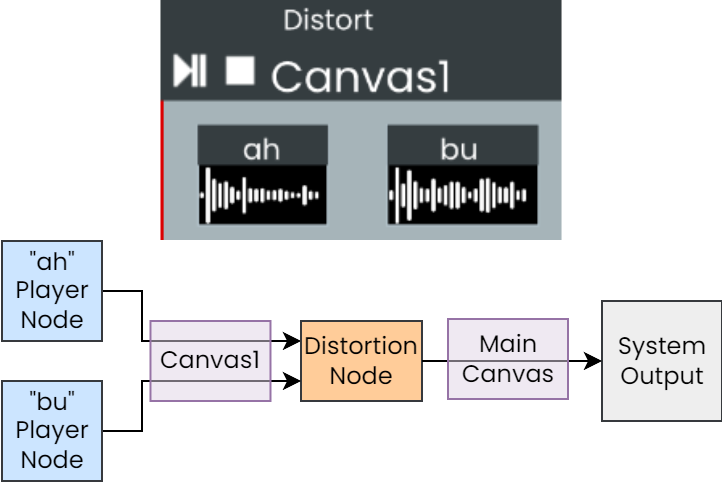
\includegraphics[scale=0.5]{images/node_diagram.png}
    \caption{An example of how ToneAudioNodes connect together and to the output in tuPAC.}
    \label{fig:node_diagram}
\end{figure}

\subsubsection{Playable}
The abstract class \playable\ has members and methods that enable objects to be played and interact with Tone. 

\begin{table}[h]
    \centering
    \begin{tabular}{c|c|p{280pt}}
        Name & Type & Description \\
        \hline
        playing & boolean & Dictates whether the \element\ is currently playing\\
        scheduleID & number & ID to track the event scheduled in Transport for the \element\ to play. This is needed to cancel and re-schedule.\\
        speed & number & The speed at which this \element\ plays. For \canvas es, this represents the amount of pixels the \timebar\ moves in 1 second.\\
        node & ToneAudioNode & The Tone node associated with this \element.\\
        startTime & number & The number of seconds after the parent \canvas\ starts playing that this \element\ should start.\\
        pauseTime & number & The current time to start from if unpaused.\\
    \end{tabular}
    \caption{Reference for the members defined by the \playable\ class.}
    \label{tab:playable_members}
\end{table}

Every time a \playable\ is placed or moved, the appropriate startTime is calculated, and then an event is scheduled on Transport to play the \playable\ at that startTime. If an existing event associated with this object is scheduled, it is cancelled using the scheduleID member.

\subsubsection{startTime calculation}
When the main \canvas\ is initialised, it is given a startTime of 0. This establishes a starting point for the whole program, as all child \playable s use the startTime of their parent to calculate their own startTime. This is necessary due to the recursive nature of the design; each \element\ has only information about itself and its direct parent. Whenever a \capsule's startTime is updated, it must update the startTime of all of its children too.

\begin{figure}[h]
    \centering
    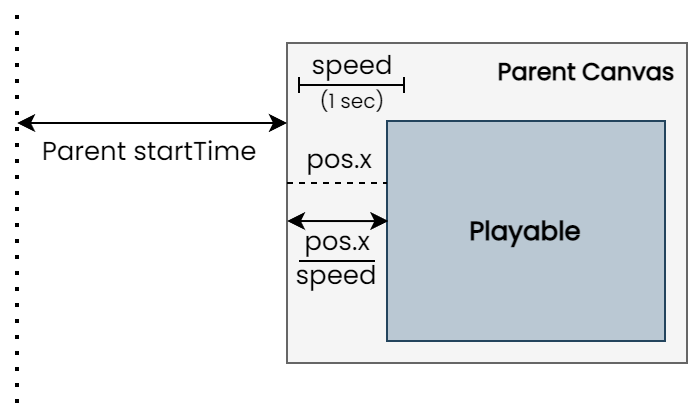
\includegraphics[scale=0.5]{images/startTime_calculation.png}
    \caption{Illustration of how the startTime of a \playable\ is calculated. The pos.x length is divided by the speed to get the duration in seconds after the parent's startTime that the \playable\ should start. Note that the speed member can be interpreted as the length in pixels passed by the \timebar\ in 1 second.}
    \label{fig:start_calc}
\end{figure}

This implementation works well as it means that at any time in the program's execution, all \playable s are correctly scheduled in the Transport's event scheduled. This means that when playing any \canvas, all that needs to be done is to play the Transport from its startTime, and to stop the Transport after it is done playing.

As the Transport deals with the timekeeping, any possible delays in the rendering of the program will not also occur in the playback of the audio. This is important for a compositional tool as precise timings may be important for the intended audio.

\subsection{Input}
The final important aspect of implementation is the user input. The class \mouse\ handles all mouse input. p5.js invokes methods when users interact with a p5 canvas. This enables tuPAC to handle input from users. In \verb|tupac.js|, there are methods to handle mouse presses, releases and key presses, as well as a single \window\ object and a single \mouse\ object. Keyboard input is passed to the \window\ object, and mouse input is passed to the \mouse\ object. The \window\ object holds a \labelT\ (or \verb|null|) and a boolean variable to represent whether the user is currently typing.

The \mouse\ object has methods which are called for each frame that is drawn, checking what is under the cursor to change it appropriately, as shown in the video submitted with the source code of the project. For example, if clicking the mouse will start typing into a \labelT, then the cursor will display as the standard cursor which represents this. 

\begin{table}[h]
    \centering
    \begin{tabular}{c|c|p{300pt}}
        Name & Type & Description \\
        \hline
        state & MouseState & The current state of the \mouse, can be any of \{free, dragging, resizingX, resizingY, resizingXY\}\\
        cursor & CursorState & The current type of cursor to draw, can be any of \{default, drag, resizeX, resizeY, resizeXY, type\}\\
        cursorOff & Pos & The offset from the cursor to the co-ordinates of the held object, used for dragging\\
        held & Element & The currently held \element, if any.\\
        lastClicked & Element & The last clicked \element, for deleting if DEL is pressed.\\
    \end{tabular}
    \caption{The members defined in the abstract \element\ class}
    \label{tab:element_members}
\end{table}

When the user clicks their mouse, a method is invoked in \mouse\ through \verb|tupac.js| which activates the relevant event. The \element\ underneath the cursor will have its \verb|clicked| method invoked, and if the cursor is in a position to begin dragging or resizing an \element, then a reference to that \element\ gets added to the \mouse's held member and the state variable changed to reflect this. Every frame, this state is checked, and the held \element\ is moved or resized appropriately. \element's moving or resizing methods may impose restrictions on these changes to ensure illegal actions don't occur. When the user releases their mouse, another method is invoked which removes any held member and changes the state back to \verb|free|.

\clearpage
\subsection{Repository overview}
This section presents an overview of the file structure of the project to conclude the chapter. All code in the \verb|src| directory was written from scratch after the research and preparation phases of the project were complete and the framework for the software was decided. The other code (the contents of \verb|main.js|, \verb|index.html|, \verb|jest.config.js| and \verb|tsconfig.json|) was written with the help of online guides, as they are somewhat generic files pertaining to Electron, Jest and TypeScript. All images used in the program are in \verb|resource/img/| and were created by me from scratch. The font stored in \verb|resource/font/| was taken from Google Fonts, under the Open Font License.

\DTsetlength{0.2em}{1em}{0.2em}{0.4pt}{2pt}
\setlength{\DTbaselineskip}{20pt}
\dirtree{%
.1 .
.1 dist/\DTcomment{The files to be run by Electron (Compiled JS files and HTML)}.
.2 index.html\DTcomment{The webpage that renders in Electron}.
.1 resource/\DTcomment{Resources other than code needed for the software}.
.2 img/.
.2 font/.
.1 src/\DTcomment{The source TypeScript files to be compiled}.
.2 capsule.ts.
.2 canvas.ts.
.2 ....
.2 tupac.ts\DTcomment{The code run in index.html to render the GUI}.
.1 test/\DTcomment{Unit tests to be run with Jest}.
.1 main.js\DTcomment{The initial code run, which opens the Electron window}.
.1 jest.config.js\DTcomment{Configuration for Jest testing}.
.1 tsconfig.json\DTcomment{Configuration for TypeScript compilation}.
}

The repository consists mainly of two folders. \verb|src| contains the TypeScript files which compile into \verb|dist|, which contains the files used at runtime. \verb|dist| also contains the HTML file which is displayed when Electron runs. The TypeScript files compile to CommonJS modules, which are imported and used by the other files. For example, the file \verb|tupac.ts| imports the module ``window", which after compilation is done by importing the \verb|window.js| file.

\chapter{Evaluation}\label{chap:eval}
As mentioned in the preparation chapter, the success of this project leans on the successful implementation of a set of features, and the extent to which it enables artists to easily create phonological compositions. In this evaluation I address the original success criteria and show that they were fulfilled. The chapter consists of analysis of the work completed, and a user study, to evaluate the \usability, \clarity\ and \expressiveness\ of the final software.

In the preparation chapter, I set out a list of possible tasks to complete for this project. \Fref[main]{tab:tasks_completed} shows all of the completed tasks, along with how we evaluate the success of each one in this evaluation.
\begin{table}[h]
    \centering
\begin{adjustbox}{center}
    \begin{tabular}{|c|c|c|c|c|}
        \hline
         Task & Priority & Difficulty & Completed? & Evaluation\\
         \hline
         Develop model of composition & \vital & \medium & \checkmark & \Fref[main]{sec:phonology}\ \&\ \Fref[main]{sec:comp_rep}\\
         \hline
         \multicolumn{5}{|c|}{Text-based tool capabilities} \\
         \hline
         Play audio & \vital & \easy & \checkmark & \inspect\\
         Represent model & \vital & \medium & \checkmark & \Fref[main]{sec:comp_rep}\\
         Apply effects to audio & \interm & \easy & \checkmark & \inspect \\
         Mapping IPA characters to samples & \extension & \medium & \checkmark & \inspect\\
         \hline
         \multicolumn{5}{|c|}{Graphical tool capabilites} \\
         \hline
         Build responsive GUI & \vital & \medium & \checkmark & \user\\
         Play audio loaded from file & \vital & \medium & \checkmark & \inspect\\
         Represent model & \high & \veryhard & \checkmark & \user\\
         Ensure time keeping of audio & \high & \hard & \checkmark & \user\\
         Apply effects to audio & \interm & \hard & \checkmark &\inspect\\
         Adjust playback speed for audio & \low & \medium & \checkmark &\inspect\\
         \timebar\ Translation & \extension & \hard & \checkmark & \inspect\\
         \hline
    \end{tabular}
\end{adjustbox}
    \caption{The tasks completed from \Fref[main]{sec:req_anal}.}
    \label{tab:tasks_completed}
\end{table}
\section{Functionality}\label{sec:func}
In order to show the objective success of the project, I show that each of the above tasks was completed in this section by presenting images of the project, as well as a video recording of tuPAC in action, included in the source code submission.

\subsection{Text-based tool}
\underline{Play audio, apply effects to audio}

The functionality of the text-based tool is demonstrated in the video submitted with the source code of the project. This shows the functionality described in the implementation chapter.

\underline{Mapping IPA characters to samples}

As this tool was made to be demonstrative, there was no need to implement this for the entire International Phonetic Alphabet, but a small subset of characters were made to easily be transformed into audio samples, recorded by myself. This is again shown in the video submitted.

\subsection{Graphical tool - tuPAC}
\underline{Build responsive GUI, play audio, represent model, apply effects, adjust playback speed}

\Fref[main]{fig:tupac_gui} shows the GUI of the graphical tool as implemented, reflecting the design in \Fref[main]{sec:final_design}. This figure and the video show the GUI was implemented, and that it is responsive running on my machine. This design was specifically built to represent the model of composition. The user questionnaire answers also demonstrate the GUI's responsiveness and the success of the compositional model's representation.

\begin{figure}[h]
    \centering
    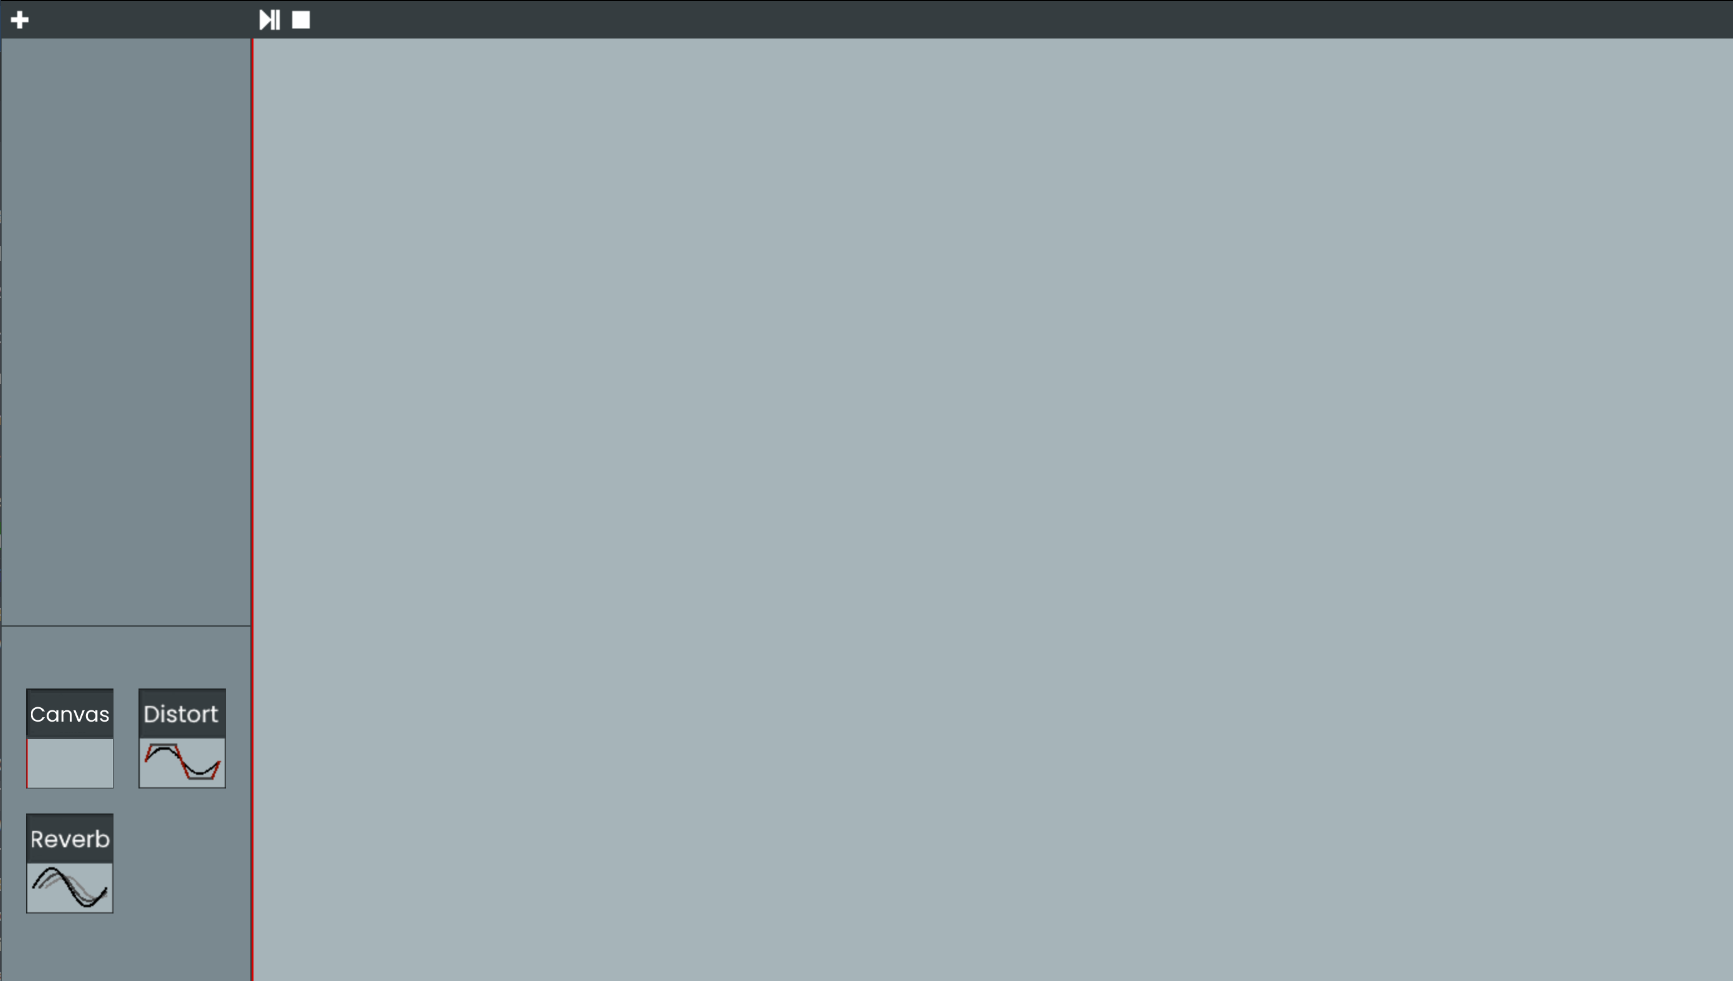
\includegraphics[scale=0.3]{images/tuPAC_GUI.png}
    \caption{The GUI of tuPAC, as is when the program is first started.}
    \label{fig:tupac_gui}
\end{figure}

\section{User Testing}
In \Fref[main]{sec:req_anal}, I defined the desirable qualities of the final project as \usability, \clarity\ and \expressiveness. In order to evaluate the extent to which tuPAC exhibits these qualities, a user study was carried out.

\subsection{Methodology}
Due to the inclusion of human participants, I was required to request a review by the Ethics Committee, which I did so successfully. As mentioned, it was deemed infeasible to gather artists to participate in this study, so general users were sought out. These participants were recruited by myself, to fit the necessary criteria:
\begin{itemize}
    \item Participants should not have difficulty using computers in general.
    \item Participants should have little to no experience using a DAW - otherwise, these users would have more overall experience with the design of a DAW than that of tuPAC when completing the tasks.
    \item Participants should consent to taking part in the study, including completing the tasks given to them and completing a questionnaire afterwards, given full disclosure of the details of the study beforehand, and that no personal data is kept.
\end{itemize}

In order to recruit users, I approached some students and asked whether they fit the criteria, and whether they were willing to participate in the study. I gathered 6 participants who met the criteria.

For each participant, I taught them the necessary functionality of both tuPAC and Ableton Live to complete a set of tasks. After learning to use a program, the user then completed the tasks in that program, before moving on to the next program. In order to control for the learning bias, half of the users started with Live, and half with tuPAC.

While users completed tasks, I recorded the time passed from starting the task to achieving a satisfactory result, in seconds. This data is presented in \Fref[main]{sec:data} as a quantitative comparison between tuPAC and Live. This type of evaluation is known as A/B testing, and is one of the most popular styles techniques used in the evaluation of NIME (New Interfaces for Musical Expression) \cite{Huot15}. After using both programs, the users completed a questionnaire, supplying qualitative assessments of both programs.

\subsection{Set-up}
In order to reflect the same set-up in both programs, I imported the files for the users prior to their completion of the tasks in both. The audio files were recorded by myself, with the names representing the sounds I made. The files were named: \verb|ah, anybody, ar, bu, du, ss, th| and \verb|the|.

\subsection{Familiarity}
Before completing the tasks in a program, it was important to build some familiarity with it. Therefore, users were demonstrated the functionality necessary to complete the tasks, and asked to complete two simple untimed tasks before the main ones. The functionality taught was:
\begin{itemize}
    \item Adding files to the timeline/canvas.
    \item Starting/stopping playback.
    \item Removing elements from the timeline/canvas.
    \item Adding effects to audio.
    \item (Live) Adding tracks.
    \item (Live) Changing the pitch of audio clips.
    \item (tuPAC) Adding canvases.
    \item (tuPAC) Changing the duration of a canvas.
\end{itemize}

After being demonstrated these features of the program, users were asked to play a sample, then play it with an effect, and then reset the program back to how it was before. This was untimed, to get users familiar with the basics of the programs.

\subsection{Tasks}
There were four tasks completed by users, which represent four different levels of difficulty of tasks that users of tuPAC might want to complete. These are referred to by the names ``Words", ``Effects", ``Layering" and ``Piece".

\subsubsection{Words}
The first task was to have two words play, bass and bath, pronounced with the same ``a" sound (/a/ in IPA). This was done by arranging the sound files into the correct order and having them play back. This task simply tested the ability of the users to have audio files play with correct timing in the programs.

\subsubsection{Effects}
This task built on the previous one. Starting with the words bass and bath already made, users had to have the word bass play with the distortion effect applied, and the word bath play with the reverb effect applied.

\subsubsection{Layering}
This task required users to have the sounds \verb|bu.wav| and \verb|ah.wav| to play, in that order. During the same amount of time, the sound anybody should also play. This task tested the users' ability to speed up or slow down audio. I chose this task in particular to evaluate the \usability\ and \clarity\ of the time bar translation described in \Fref[main]{sec:timebar_translate}.

\subsubsection{Piece}
The final task combined the skills learnt in such a way that reflects a more complex endeavour in the programs, within the scope of users' abilities after only a little practice. The task is completed in the video associated with this dissertation. Users had to create the sentence ``the bad are", where only the word ``bad" had the distortion effect applied to it. For the duration of this sentence playing, the word ``anybody" should repeat underneath it. The result in tuPAC should be similar to that shown in \Fref[main]{fig:canvas_tree}.

\subsection{Questionnaire}
The questionnaire was hosted on Google Forms, making anonymous data collection easy. I was able to send each participant a link to the questionnaire and have them complete it right after participating in the study.

The questionnaire consisted of four sections, two for each program. In the first section for each program, participants were provided a sequence of sentences, and asked to select one of 5 options, ranging from ``Strongly Disagree" to ``Strongly Agree". This is known as a \textbf{Likert scale}, a well-documented method of measuring people's attitudes to a given statement \cite{Likert32}. The second section consists of a few longer form questions, where participants were given a text box to provide comments on specific aspects of the program.

\subsection{Qualitative Results}\label{sec:qual_res}
In the second part of the questionnaire, participants were asked the following questions about both programs:

\quoteT{To what extent did the program effectively help you carry out the tasks you were given today? What aspects of the program's design helped you and what hindered you?}

\quoteT{What features (if any) would have greatly improved your experience using the program?}

\quoteT{How well did you understand the interface of the program? Were there significant features/portions of the layout which weren't clear in their purpose/significance? (If so, please explain)}

These questions aimed to get specific feedback on what worked well and what didn't work well when completing the given tasks in each program. It is important to note that these users were recruited by myself, and could have a bias towards my software, but participants were asked to answer truthfully and had nothing to gain from doing otherwise. Also note that all quotes are presented as written by the participants, some with grammar/spelling mistakes.\footnote{The most relevant quotes are presented here to keep the section succinct but the rest of the responses can be found in \Fref[main]{appendix:raw}, if desired.}

\subsubsection{Usability}
For the first question, participants were able to express specific opinions on the usability of the software. 

About \textbf{Live}, one participant wrote \quoteT{The features I needed were in places I \textbf{didn’t really think made sense}. I knew where they were after being given an explanation, but without that I think I would have had to search for a while.} This sentiment is reflected in \Fref[main]{fig:q_leg} and in the third question of this section. 

In comparison, participants wrote about \textbf{tuPAC} \quoteT{the lack of constraints in where I placed the clips meant it was easier to link together sounds, forming full words.} and \quoteT{I also liked that you could \textbf{place clips exactly where you want to place them (not snapped to a grid) and I think this is especially advantageous when using voice clips.}} These quotes highlight the \usability\ of tuPAC's design when compared to Live's in phonological composition tasks - especially the last quote, which supports tuPAC's superiority when arranging audio in these tasks.

Three participants found that the implementation of clip arrangement in \textbf{Live} was cumbersome in the execution of the given tasks. \quoteT{The program helped me carry out the tasks, but I was hindered by the design of \textbf{how hard it was to drag sounds} and to find each effect.}

Another shared sentiment was the difficulty of changing the duration of sound clips. \quoteT{I thought the use of \textbf{a rotary encoder to specify pitch was very difficult to use}, due to the size of it making small adjustments to the mouse position have a big effect on the pitch.}, \quoteT{it seemed long winded on how to apply effects and felt like there could be an easier way to do it. i feel the same way regarding the lengthening of sounds. \textbf{it was challenging}.} This highlights the \textbf{benefit felt from the intuitiveness} of the time bar translation in \textbf{tuPAC}.

\subsubsection{Functionality/Expressiveness}\label{sec:qual_funct}
Functionality is a lot more straight forward. For both programs, a few participants had no suggestions on missing functionality.

One participant suggested for \textbf{Live} \quoteT{A better method of adjusting pitch.}, which seems to have been a common issue during this evaluation, as this answer also points out, \quoteT{Freedom in clip movement and \textbf{an easier way to change clip length.}}

For \textbf{tuPAC}, one participant suggested two good features which could be implemented in further work to improve the functionality of the system: \quoteT{A copying feature may be useful in duplicating words. A selection box to move multiple clips at once.}

\subsubsection{Clarity}
All participants gave positive responses on the legibility of \textbf{tuPAC}, suggesting a great success in the \clarity\ of the design of tuPAC for phonological composition structures.


\quoteT{I understood the interface \textbf{perfectly}}

\quoteT{I felt \text{I understood it well}. I don’t think anything wasn’t clear in its purpose.}

This was contrasted with general complaints about \textbf{Live}'s interface. Only one participant had a purely positive response about Live: \quoteT{The interface was clear.}

%\quoteT{\textbf{More confusing to understand}, for example making the length of the sample change was \textbf{less intuitive} .}

\quoteT{The interface felt quite \textbf{cluttered and unintuitive}}

%\quoteT{I felt I understood it fairly well, but it \textbf{looked very cluttered}. (...)}

\subsection{Quantitative Results}\label{sec:data}
This section presents the results from the user study and uses them to evaluate the success of the project.

\subsubsection{Tasks}
First, we see a box plot of each task performed in each program.

\begin{figure}[h]
    \centering
    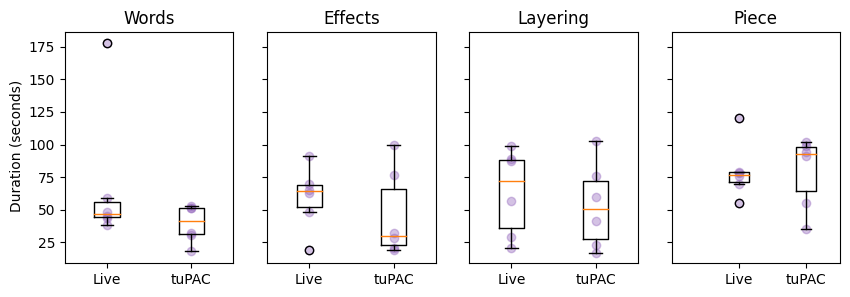
\includegraphics[width = .9\linewidth]{images/box_plot.png}
    \caption{Box plot of timing data.}
    \label{fig:box_plot}
\end{figure}

This plot shows us that \textbf{tuPAC generally outperformed Live} in users' time taken to complete the tasks. In the Piece task, the median is slower for tuPAC, but we can see that two out of the six participants completed it much faster. This plot doesn't tell the whole story of the study, as participants were split into two groups. Whether participants completed the tasks in Live or in tuPAC first was a major factor in their results. Due to this and the small sample size, it is useful to see what individual participants achieved, and this can be seen in \Fref[main]{fig:change_per_task}.

\begin{figure}[h!]
    \centering
    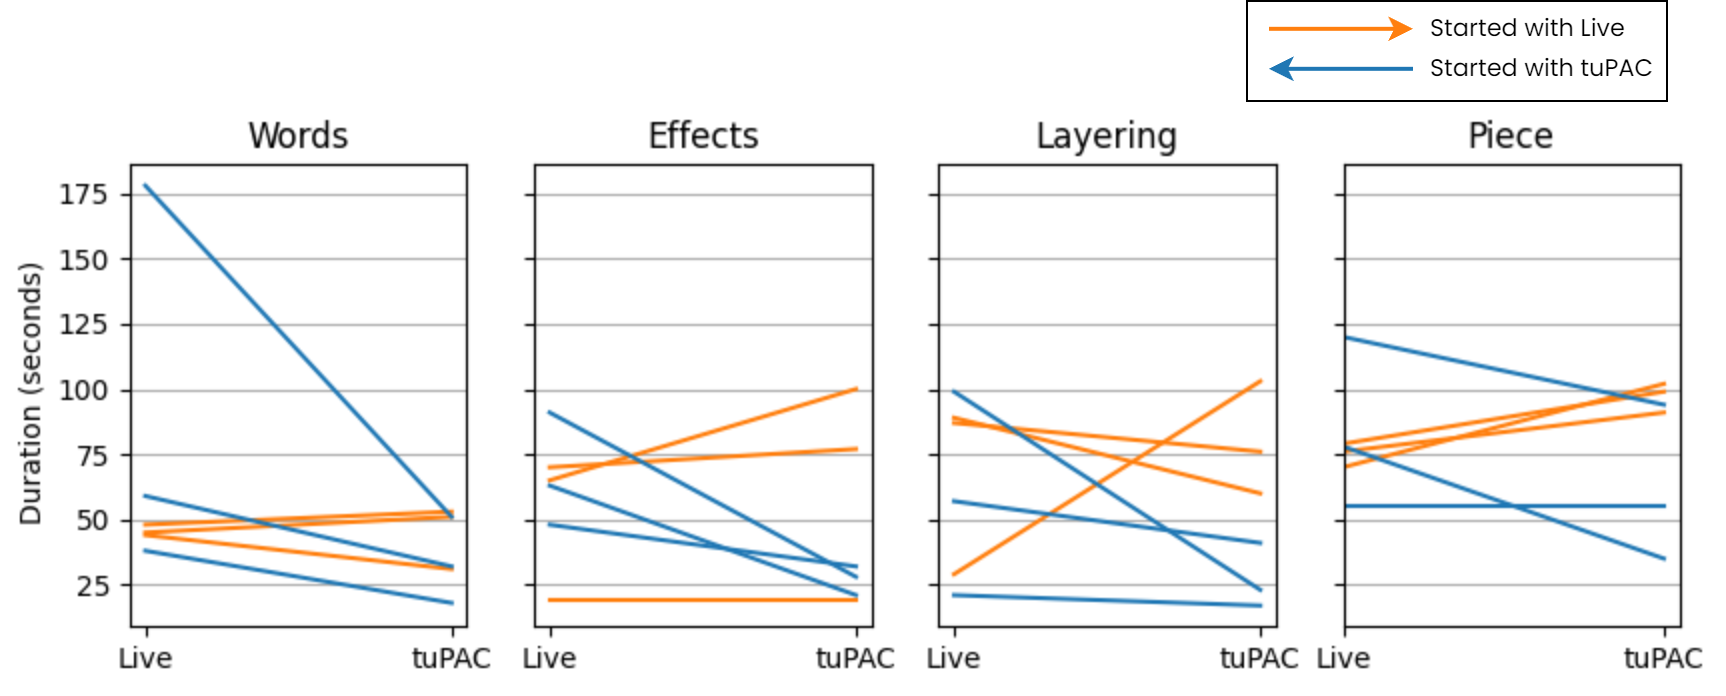
\includegraphics[scale=0.25]{images/time_data.png}
    \caption{The time taken for participants to complete each task in each program separated by task. The four charts show the time taken in the ``Words", ``Effects", ``Layering" and ``Piece" task from left to right.}
    \label{fig:change_per_task}
\end{figure}


Inspection of \Fref[main]{fig:change_per_task} shows that \textbf{when starting with Live}, the participants  \textbf{significantly improved their time when switching to tuPAC}, and that this was not the case when participants started with tuPAC and switched to Live.

\subsubsection{Questionnaire - Likert scale}
The questionnaire results are presented in this section, grouped together by the aspects that they evaluate.

\begin{figure}[h!]
\centering
\begin{subfigure}{.5\textwidth}
  \centering
  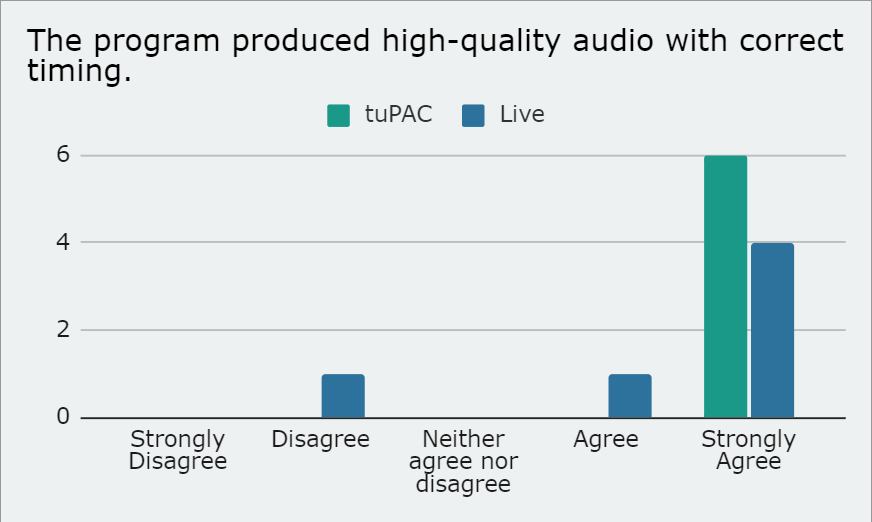
\includegraphics[width=.9\linewidth]{images/questionnaire/functionality.png}
  \caption{Output}
  \label{fig:q_funct}
\end{subfigure}%
\begin{subfigure}{.5\textwidth}
  \centering
  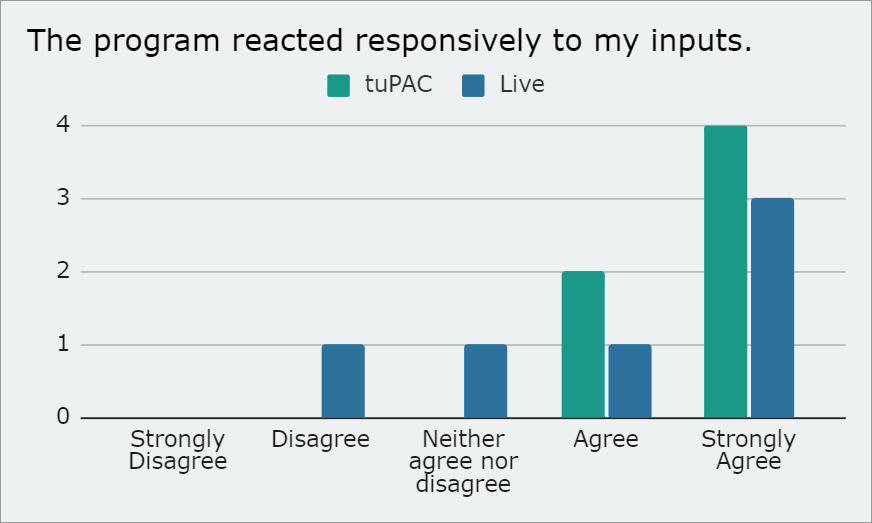
\includegraphics[width=.9\linewidth]{images/questionnaire/responsiveness.png}
  \caption{Responsiveness}
  \label{fig:q_resp}
\end{subfigure}
\caption{Charts showing users' evaluations of the practical usage of both programs.}
\label{fig:q_1}
\end{figure}

\begin{figure}[h!]
\centering
\begin{subfigure}{.5\textwidth}
  \centering
  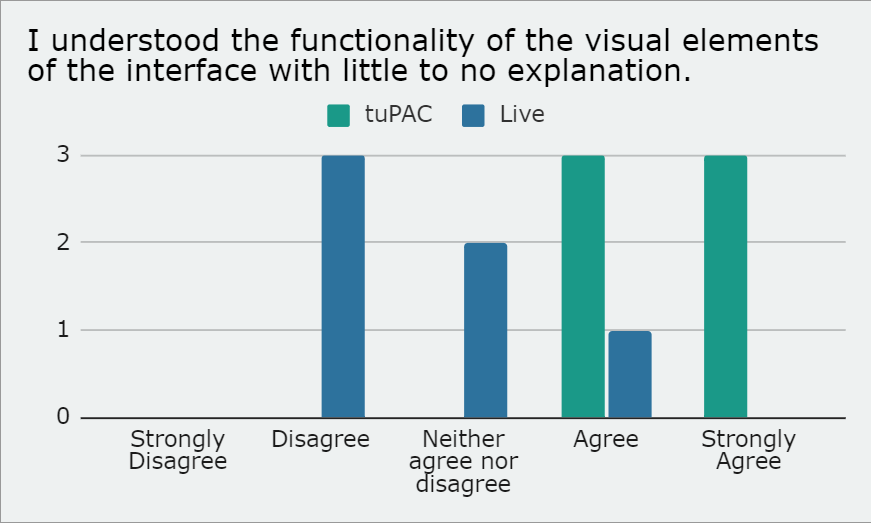
\includegraphics[width=.9\linewidth]{images/questionnaire/intuitiveness.png}
  \caption{Intuitiveness}
  \label{fig:q_intu}
\end{subfigure}%
\begin{subfigure}{.5\textwidth}
  \centering
  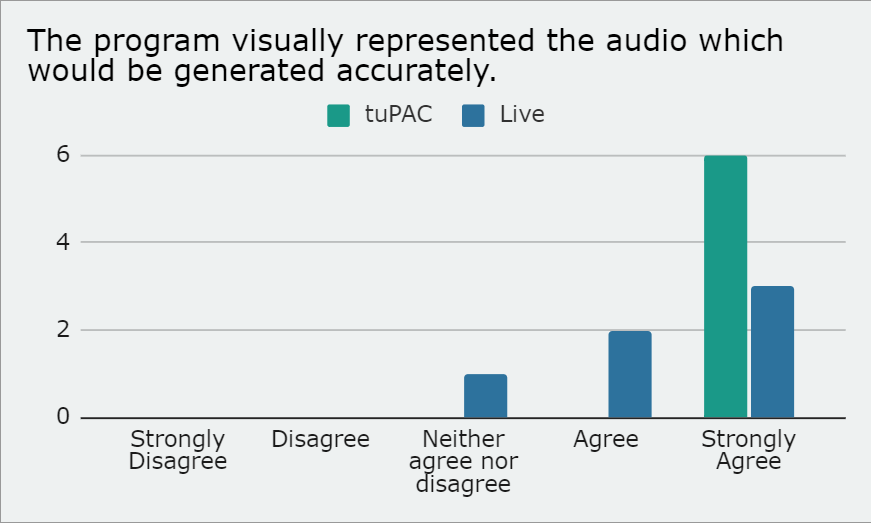
\includegraphics[width=.9\linewidth]{images/questionnaire/visual_correspondence.png}
  \caption{Visual Correspondence}
  \label{fig:q_corresp}
\end{subfigure}
\caption{Charts showing users' evaluations of the visual \clarity\ of both tools.}
\label{fig:q_2}
\end{figure}

\begin{figure}[h!]
\centering
\begin{subfigure}{.33\textwidth}
  \centering
  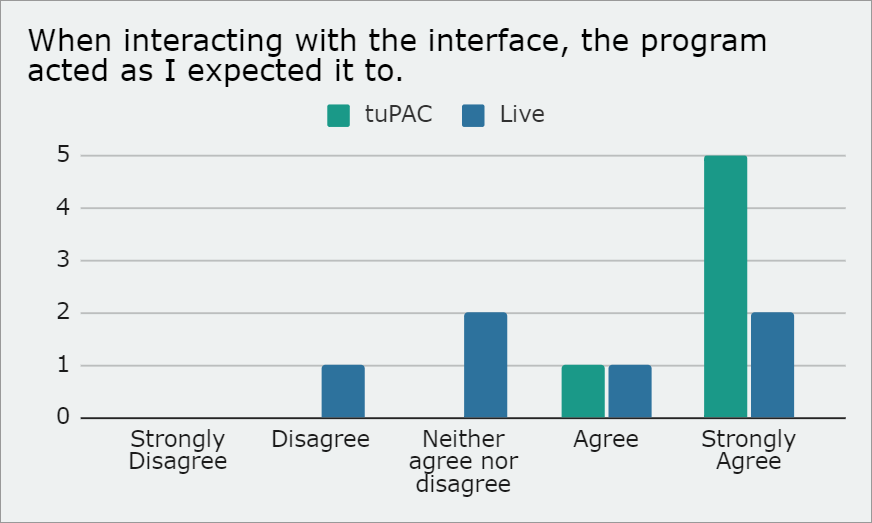
\includegraphics[width=.9\linewidth]{images/questionnaire/predictability.png}
  \caption{Predictability}
  \label{fig:q_predict}
\end{subfigure}%
\begin{subfigure}{.34\textwidth}
  \centering
  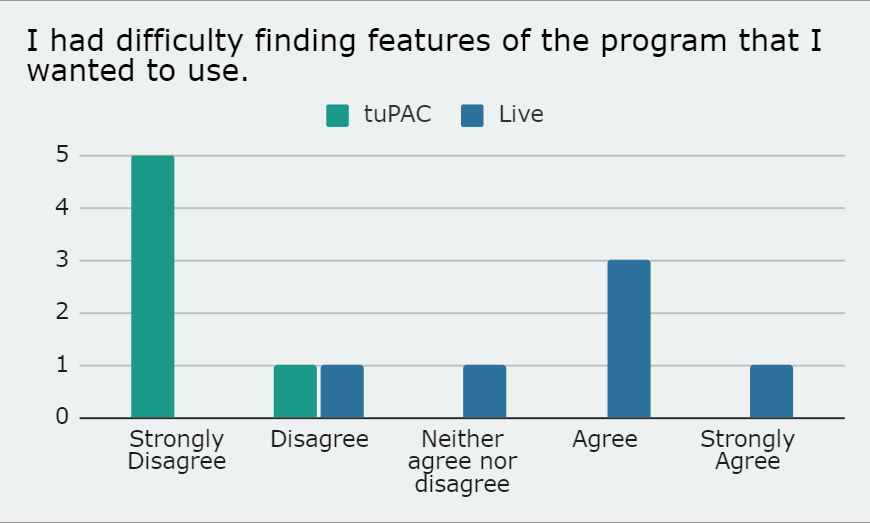
\includegraphics[width=.9\linewidth]{images/questionnaire/legibility.png}
  \caption{Legibility}
  \label{fig:q_leg}
\end{subfigure}%
\begin{subfigure}{.33\textwidth}
    \centering
    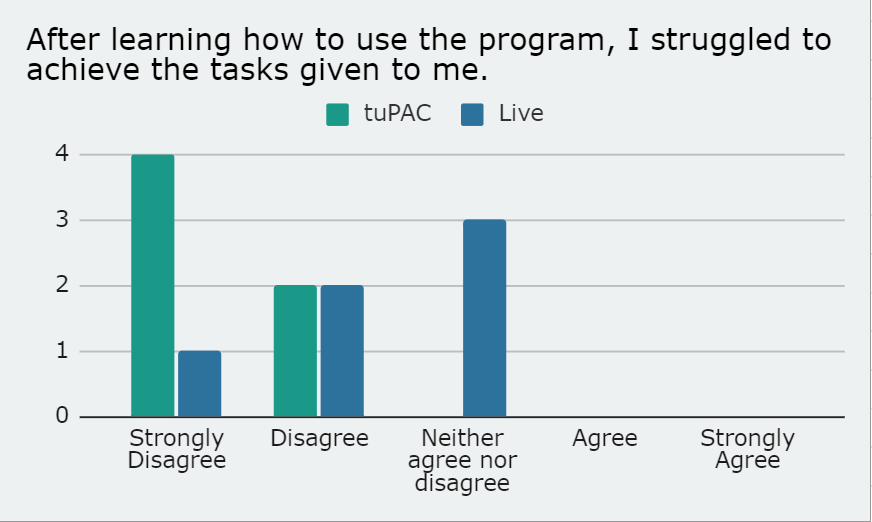
\includegraphics[width=.9\linewidth]{images/questionnaire/usability.png}
    \caption{\Expressiveness}
    \label{fig:q_expr}
\end{subfigure}
\caption{Charts showing users' evaluations of the \usability\ and \expressiveness\ of both programs.}
\label{fig:q_3}
\end{figure}



\clearpage
\subsubsection{Summary of quantitative data}
\statement{\Usability: The ability for the program to actualise the user's intentions by making common actions fast and intuitive.}

When completing tasks pertaining to phonological composition, users \textbf{greatly improved} their time-to-complete when moving \textbf{from Live to tuPAC}, but only \textbf{marginally improved} when moving \textbf{from tuPAC to Live}. This is displayed in \Fref[main]{fig:change_per_task}.

tuPAC scored far better on the statements in \Fref[main]{fig:q_predict} and \Fref[main]{fig:q_leg}, meaning \textbf{users found tuPAC much easier to understand and navigate than Live} in the tasks they were given.

\statement{\Clarity: A clear correspondence between what happens on the screen, and what the user imagines is happening to their composition. When the user makes a change, the program changes the audio appropriately, in line with the user's expectations.}

The design of tuPAC was based on a model of composition developed through correspondence with an artist. This ensured a fluent visual correspondence between cognitive structures found in phonological composition and tuPAC's GUI. Users \textbf{rated tuPAC better than Live} in the three statements (\Fref[main]{fig:q_2} and \Fref[main]{fig:q_expr}) which related to the \clarity\ of the programs.

\statement{\Expressiveness: The user is not limited in what they are able to do, and can achieve whatever they would like to do with the program.}
All core features were implemented into the system (\Fref[main]{sec:func}). The \timebar\ translation feature was also implemented as an extension. We can see that users were content with the \expressiveness\ of tuPAC, as they did not struggle to complete the tasks given to them (\Fref[main]{fig:q_3}). Furthermore, they \textbf{rated Live less favourably} in this statement, finding \textbf{Live generally more difficult} than tuPAC to complete the tasks.

\chapter{Conclusions}
The aim of this project was to design and develop a novel system to provide an alternative to modern digital composition techniques, improving the process for particular styles of composition. This was completed in three stages: the development of a computational model of composition, a demonstrative text-based tool to refine the ideas for the final platform, and a graphical user interface for phonological audio composition, based on the information gathered in the first two stages. These three stages were completed successfully, resulting in a digital composition platform which can be used freely for artists to explore new musical expressions.

\section{Results}
The project was a great success. It delivered tuPAC, an \textbf{accessible, intuitive graphical interface} capable of producing \textbf{high-fidelity audio}, which is publicly available through a GitHub repository. A user study was carried out which showed \textbf{tuPAC's superiority} in terms of \usability, \clarity, and \expressiveness\ over Ableton Live - an industry-standard solution for digital composition - when executing tasks related to phonological composition. tuPAC provides an \textbf{easy-to-understand notation for phonological composition} for artists; it supplies a \textbf{malleable visual representation} which corresponds to the \textbf{structures used in these types of composition, by design}.

\section{Lessons Learned}
Throughout the research and development of this project, I learned many important lessons. Firstly, I learned and reinforced the importance of planning and design in the development of user interfaces. If it wasn't for the research and development that went into the text-based tool in the first stage of the project, I wouldn't have been able to achieve what I did with the final system. If I had designed the interface based on my own intuition without correspondence with an artist, I could have gotten too deep into implementation before noticing major issues in the \usability\ or \clarity\ for tasks that the software should aim to support. 

I also learned the importance of testing that functionality works how you intend to use it in a project before relying on it. Open source API references are not always completely accurate. This also solidified the importance of planning extra time to deal with unforeseen circumstances in the development of large projects such as this.

\section{Further Work}
This project has provided the theoretical and practical basis for further exploration into the potential of audio composition interfaces and their ability to assist in the creation of music. The design of the system provides a new approach to digital audio composition which could be developed further to inform the design of other systems, contributing to the growing range of musical software being produced. Further work could implement more features into the tuPAC software (such as those mentioned in \Fref[main]{sec:qual_funct}), or use the research and theoretical material of this dissertation in order to develop a different compositional tool.

%TC:ignore
%%%%%%%%%%%%%%%%%%%%%%%%%%%%%%%%%%%%%%%%%%%%%%%%%%%%%%%%%%%%%%%%%%%%%
% the bibliography
\addcontentsline{toc}{chapter}{Bibliography}
\printbibliography

%%%%%%%%%%%%%%%%%%%%%%%%%%%%%%%%%%%%%%%%%%%%%%%%%%%%%%%%%%%%%%%%%%%%%
% the appendices
\appendix


\chapter{Raw Participant Responses}\label{appendix:raw}

\section{tuPAC}
To what extent did the program effectively help you carry out the tasks you were given today? What aspects of the program's design helped you and what hindered you? 
\begin{enumerate}
    \item I found the canvas creation very useful, it helped me create and distort full words. In addition the lack of constraints in where I placed the clips meant it was easier to link together sounds, forming full words. For contrast in ableton, the fixed boxes were hard to move, and meant I would have to zoom in and out to obtain better flow between clips.
    \item The fact that audio clips where visually represented very differently and in a seperate section from the effects, made it easy to find what I was looking for each time. I also liked that you could place clips exactly where you want to place them (not snapped to a grid) and I think this is especially advantageous when using voice clips. The ability to just play one canvas meant I could quickly figure out if each part worked individually.
    \item The program clearly displayed the different effects and was clear on how to use it. It was very clear what effects were attached to what sounds, and what was going to be played.
    \item i liked the program. i found the canvas box challenging at first, but got used to it quickly.
    \item The ability to control distortion of specific blocks without having to create separate tracks was helpful, as there was always a visual cue highlighting the audio effects applied to each block - opposed to Ableton where this was not clear.
    \item I found that the program very effectively allowed mr to carry out the tasks I given. I found the layout of the interface very clear and easy to use, the slight problems when dragging a canvas onto an effect slightly hindered me.
\end{enumerate}


What features (if any) would have greatly improved your experience using the program?
\begin{enumerate}
    \item A copying feature may be useful in duplicating words. A selection box to move multiple clips at once.
    \item It would have been nice to be able to import multiple files or a whole directory at once
    \item Can't think of anything to improve
    \item bigger margins for sound effects to be applied.
    \item Potentially a horizontal alignment / snap to grid when aligning blocks.
    \item To have less problems when trying to drag a canvas onto an effect.
\end{enumerate}

How well did you understand the interface of the program? Were there significant features/portions of the layout which weren't clear in their purpose/significance? (If so, please explain)
\begin{enumerate}
    \item I think the interface was clearly divided into sections with different functions. It was clear where I needed to go to add clips, or add distortions, and meant it was easy to use.
    \item I understood the interface perfectly
    \item There wasn't really anything that wasn't self-explanatory.
    \item i understood it
    \item All features were clear.
    \item I felt I understood it well. I don’t think anything wasn’t clear in its purpose.
\end{enumerate}

\section{Ableton Live}

To what extent did the program effectively help you carry out the tasks you were given today? What aspects of the program's design helped you and what hindered you? 
\begin{enumerate}
    \item The fixed boxes made clip movement very hard. The separated tracks meant it was clear to split tasks up into separate parts, but when I had to change the length of sounds I had to edit each individual clip.
    \item The features I needed were in places I didn’t really think made sense. I knew where they were after being given an explanation, but without that I think I would have had to search for a while.
    \item Well laid out, automatic snapping into place helped line up sounds but there was a lot going on not as easy to find things.
    \item i did not understand the adding of effects very well. it seemed long winded on how to apply effects and felt like there could be an easier way to do it. i feel the same way regarding the lengthening of sounds. it was challenging.
    \item I thought the use of a rotary encoder to specify pitch was very difficult to use, due to the size of it making small adjustments to the mouse position have a big effect on the pitch.
    \item The program helped me carry out the tasks, but I was hindered by the design of how hard it was to drag sounds and to find each effect.
\end{enumerate}

What features (if any) would have greatly improved your experience using the program?
\begin{enumerate}
    \item Freedom in clip movement and an easier way to change clip length.
    \item It was quite hard to keep track of which effects were on each track, so a clear visual indicator for that would’ve been helpful
    \item Not sure how to improve
\item making the effects easier to find.
\item A better method of adjusting pitch.
\item If it were easier to drag sounds and find each effect.
\end{enumerate}

How well did you understand the interface of the program? Were there significant features/portions of the layout which weren't clear in their purpose/significance? (If so, please explain)
\begin{enumerate}
    \item I would search for some time, to change the length of a clip, often to find I needed to click a small tab. I dont think that the interface was intuitive, especially for someone new to audio engineering.
\item The interface felt quite cluttered and unintuitive
\item More confusing to understand, for example making the length of the sample change was less intuitive .
\item i did not like how small the sounds appeared on the screen. i felt like they could have been bigger from the start. instead you had to scroll with the control button which added time and made it less efficient.
\item The interface was clear.
\item I felt I understood it fairly well, but it looked very cluttered. There were lots of things about it that didn’t seem to serve as much purpose and could have been laid out more clearly.
\end{enumerate}


\chapter{Project Proposal}\label{appendix:proposal}

\documentclass{article}
\usepackage[utf8]{inputenc}
\usepackage{graphicx}
\usepackage[indent=0pt,skip=10pt]{parskip}
\usepackage[a4paper, total={6in,8in}]{geometry}

\begin{document}

\section*{Introduction}

There exists a wide variety of digital tools to aid the composition of music. Modern DAWs (Digital Audio Workstations) such as Ableton and Fruity Loops are used extensively in the recording, mixing and mastering of most of the music that is produced today. These applications are designed to allow musicians to easily rearrange, layer and manipulate snippets of audio which can be imported from external sources, recorded onto the tracks or generated by MIDI instruments. While this design makes musical composition and recording simple and accessible for many popular styles of music, it can be restricting to other styles of composition and inhibit explorations into more niche musical expressions. 
\begin{figure}[h]
    \centering
    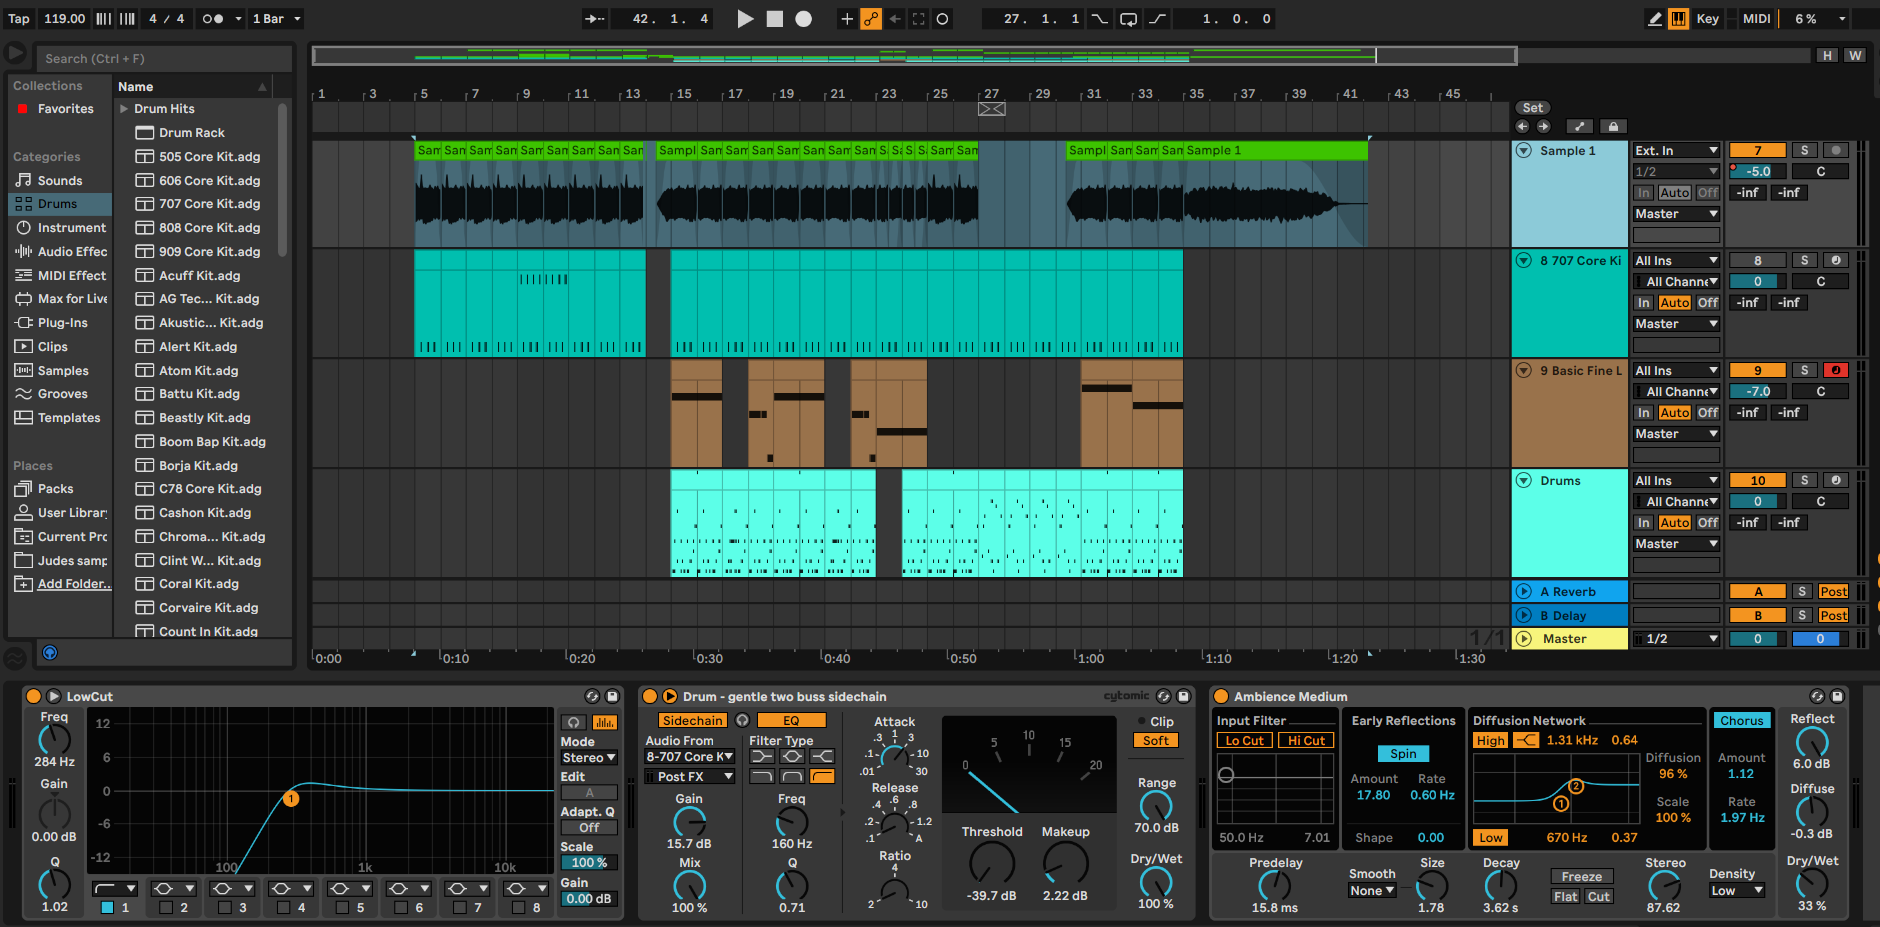
\includegraphics[scale=0.3]{images/ableton example.png}
    \caption{An example of an industry-standard DAW (Ableton 11)}
    \label{fig:ableton}
\end{figure}

Another style of digital music composition that is particularly relevant to my project is through live coding techniques. Live coding (with regards to musical composition) is a performance art in which the artist types code in front of an audience, into an environment which translates the code into music.

TidalCycles is one such platform. Tidal is software which allows people to create music through programming. Users create rhythmic patterns and generate sounds from synths or play samples as dictated by these patterns. It is embedded in the Haskell programming language and uses a custom synth and sampler called SuperDirt, built on the SuperCollider platform.

For my project, I will create an interactive music composition tool which facilitates the composition of music using speech sounds. These sounds may be generated digitally or from small samples of real recordings. I will build a text-based tool on top of an existing text-based audio generation platform (Strudel or Sonic Pi) which will allow users to create music from small literals representing snippets of speech, as well as a graphical user interface which allows users to rearrange and connect blocks to generate audio, in a style similar to the popular visual programming language Scratch.

Strudel is a web-based live coding environment intended to replicate the ideas of TidalCycles, but instead built on JavaScript and run in a browser. It uses a few different browser-available playback methods, most notably the Web Audio API and Tone.JS. There is a work-in-progress feature which allows it to communicate with SuperCollider and run SuperDirt.
\begin{figure}[ht]
    \centering
    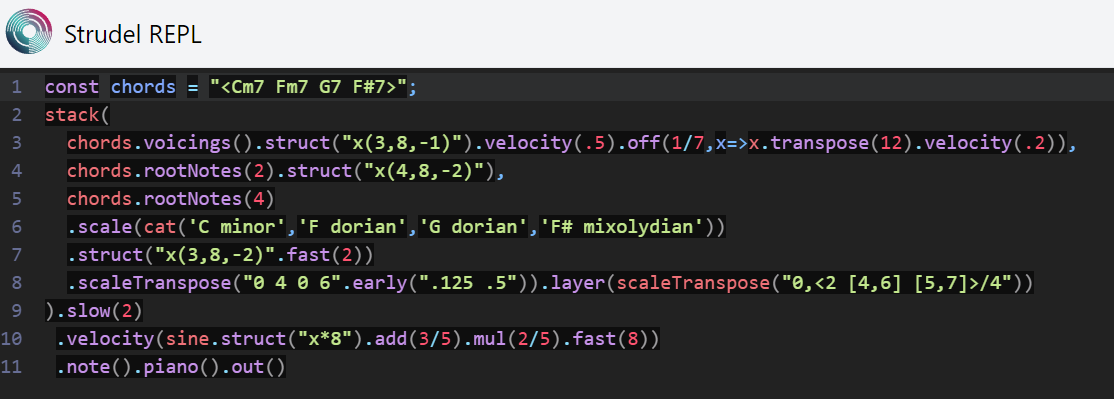
\includegraphics[scale=0.5]{images/strudel.png}
    \caption{The Strudel REPL (web-based application which runs Strudel), with example code/music}
    \label{fig:strudel}
\end{figure}

Another example of a live coding platform that I could work with is Sonic Pi, which is a standalone application with a much simpler language to write music and more in-depth tools than Strudel, but it is more limiting in the ease of expressiveness of the language. It is written in C++ and Ruby. It also uses SuperCollider to generate audio.
\section*{Starting Point}
I have very little experience with live coding and digital audio generation. I have no experience working in JavaScript or Ruby. I will need to learn about how Strudel and Sonic Pi work during the project, and will need to learn how to work with JavaScript or Ruby.
\section*{Substance of Project}
\subsection*{Core}
I will produce a piece of software which allows users to write code and generate audio from speech sounds in order to create music. Users will be able to take small snippets of speech and combine them by playing them back in a chosen order, with a chosen rhythm, by layering them, and by manipulating them in various ways.

I will also produce a piece of software which allows user to achieve a similar goal through diagrammatic means. A GUI will allow a user to take small speech literals as blocks and order them, pass them through filters, layer them or loop them.

Although tools exist that already allow you to do what my project will achieve, it will greatly improve the efficiency for a style of composition which, to my knowledge, has no tools dedicated to enabling it. You can achieve what my project will achieve in a standard DAW, but my tool will allow users to achieve more complicated rhythms and structures in much less time than they would moving samples of speech around in a DAW. It also makes the process much more accessible, allowing users with little experience working with digital composition tools or with programming to work with this style of proposition and to work with live coding techniques.
\subsection*{Extensions}
Some possibles extensions of my project would:
\begin{itemize}
    \item Build an explicit formal language describing the composition and generation of audio, based on the text-based tool.
    \item Change the text-based tool to reflect the definition of the formal language.
    \item Change the graphical tool to represent this formal language.
    \item Integrate neural synthesis of speech sounds into my composition tool. Antoine Caillon and Philippe Esling released a paper last year detailing a variational auto-encoder they have developed (RAVE) which allows for fast, high quality audio synthesis. I could implement RAVE into the tool to allow users to generate their own speech audio with state-of-the-art neural synthesis, adjusting parameters to change the sound in real time.
\end{itemize}
\section*{Success Criterion}
In order to have succeeded in my project, I require:
\begin{itemize}
    \item Software which allows users to write code which will use speech sounds to generate an audio output.
    \item Software which allows users to rearrange blocks specifying speech sounds and operations on those sounds in order to generate an audio output.
    \item Both pieces of software should allow for users to:
    \begin{itemize}
        \item Play back a small sample of speech.
        \item Arrange multiple sounds to be played back with a particular rhythm and order.
        \item Layer multiple sounds to be played alongside each other.
        \item Manipulate sounds with filters and effects.
    \end{itemize}
    \item The software be evaluated against an industry-standard DAW in user tests to express the efficacy of both the graphical and text-based tool in the production of phonological music.
\end{itemize}
For the final bullet point, I will supply the software to users who will give written feedback on the ease of use of my tool and existing tools. I will also measure the time taken for users to complete specific tasks to measure quantitatively the improvement on certain tasks over existing tools. I will use A/B testing to compare the two implementations, text-based and graphical, to measure the ease of use for each tool.
\section*{Timetable}
\subsection*{Feedback}
Over the duration of my project, I plan to interact with users for feedback. I am already in contact with one artist and I will venture to find other possible users of my tool through people I know and get feedback from a wider source. In the first few weeks, I will need to fill in the form for the Ethics Committee to approve the involvement of human participants.
\subsection*{Week 1/2: 16th Oct. - 29th Oct.}
\begin{itemize}
    \item Study Strudel framework.
    \item Study Sonic Pi framework.
    \item Set up work environment for development of text-based tool.
\end{itemize}
{
\centering\textbf{Milestone:} Decide whether to work with Strudel or Sonic Pi, supplying a report describing the details of the research and my choice to my supervisor. Be able to compile and run Strudel and/or Sonic Pi on my own machine, allowing for my own modifications and additions to the code.
}
\subsection*{Week 3/4: 30th Oct. - 12th Nov.}
\begin{itemize}
    \item Research system for generation of audio.
    \item Understand how to generate, combine and manipulate audio to produce new outputs.
\end{itemize}
{
\centering\textbf{Milestone:} Write program which is able to generate sample audio outputs, working on samples given by user.
}
\subsection*{Week 5/6: 13th Nov. - 26th Nov.}
\begin{itemize}
    \item Begin programming of text-based composition tool.
\end{itemize}
{
\centering\textbf{Milestone:} Have functioning text-based tool which allows users to input code and generate audio using small snippets of speech.
}
\subsection*{Week 7/8: 27th Nov. - 10th Dec.}
\textit{Michaelmas term ends: 1st Dec. Varsity skiing trip}
\begin{itemize}
    \item Continue work on text-based tool.
    \item Test text-based implementation on user, get feedback.
\end{itemize}
{
\centering\textbf{Milestone:} Report describing user feedback, possible improvements and tweaks to system.
}
\subsection*{Week 9/10: 11th Dec. - 24th Dec.}
\begin{itemize}
    \item Refine text-based tool based on feedback.
\end{itemize}
{
\centering\textbf{Milestone:} New, improved version of tool modified based on the feedback from the user.
}
\subsection*{Week 11/12: 25th Dec. - 7th Jan.}
\textit{Christmas and New Years Eve, will not be completing much work.}
\begin{itemize}
    \item Research libraries for creating visual programming languages (e.g. Blockly).
\end{itemize}
{
\centering\textbf{Milestone:} Write up a page for project supervisor describing what I have learnt, what library I will use and how I will use the library to create a GUI.
}
\subsection*{Week 13/14: 8th Jan. - 21st Jan.}
\textit{Lent term starts: 17th Jan.}
\begin{itemize}
    \item Build diagrammatic tool for phonological audio composition.
\end{itemize}
{
\centering\textbf{Milestone:} Working GUI, allowing users to rearrange blocks in order to generate audio in different ways.
}
\subsection*{Week 15/16: 22nd Jan. - 4th Feb.}
\textit{Progress deadline due: 3rd Feb (12pm)}
\begin{itemize}
    \item Feedback from user.
    \item Improve on GUI.
    \item Write progress report.
\end{itemize}
{
\centering\textbf{Milestone:} Hand-in progress report, written evaluation of user feedback.
}
\subsection*{Week 17/18: 5th Feb. - 18th Feb.}
\begin{itemize}
    \item Start writing the dissertation.
\end{itemize}
{
\centering\textbf{Milestone:} Complete draft chapter to be reviewed by project supervisor.
}
\subsection*{Week 19/20: 19th Feb. - 4th Mar.}
\textit{Slack: time for me to catch up if running behind, complete extensions if ahead.}
\subsection*{Week 21/22: 5th Mar. - 18th Mar.}
Continue to write dissertation.

{
\centering\textbf{Milestone:} Draft of Introduction, Preparation chapters to be sent to supervisor.
}
\subsection*{Week 23/24: 19th Mar. - 1st Apr.}
Continue to write dissertation.
{

\centering\textbf{Milestone:} Draft of Implementation, Evaluation chapters to be sent to supervisor.
}
\subsection*{Week 25/26: 2nd Apr. - 15th Apr.}
Continue to write dissertation.

{
\centering\textbf{Milestone:} Full draft of dissertation to be sent to supervisor.
}
\subsection*{Week 27/28: 16th Apr. - 29th Apr.}
\textit{Slack: time for me to push back goals into.}
\subsection*{Week 29/30: 30th Apr. - 12th May}
\begin{itemize}
    \item Final touch-ups.
    \item Hand in final dissertation.
\end{itemize}
{
\centering\textbf{Milestone:} Finish project!
}

\textit{Note: During the weeks of writing the dissertation, I will periodically be sending the drafts to my supervisor for feedback, and improving on them when feedback is received.}
\section*{Resource Declaration}
My own laptop is sufficient to complete this project. No particularly heavy computation will be necessary. I don't have much storage left on my laptop, so I will need to acquire an extra SSD. The software and libraries that I will be using in this project is all publicly available (Strudel, Blockly, Sonic Pi, SuperDirt,  etc.). I will use a GitHub repository to store my code as well as my own laptop storage, and so in case of a failure of my laptop I will have a back-up of my work.
\textit{I accept full responsibility for this machine and I have made contingency plans to protect myself against hardware and/or software failure.}
\end{document}

%TC:endignore
\end{document}